\cotefile{150}
\scanpage{85}
\mspage{\uline{16}}

\[\Sigma_J\sim\Sigma_{J,L}.\]

\margin{Un point de vue peut-être plus commode pour définir les $\Sigma_i$, $\Sigma_{i_0\ldots i_n}$, $\Sigma_J$, $\Sigma_J^{\unsure{L|*}}$ est celui des ``\unsure{éclatés orientés}'', mieux adapté à des formules du type $X=\underset{d\in\mathrm{Drap}(I)}{\lim}\Sigma_d$. On prend des $\Sigma_i\supset X_i^*$ et \unsure{non} $\deleted{\unsure{\Sigma_i}}\subset X_i^*$, \unsure{idem pour} $\Sigma_J$, $X_J^*=\Sigma_J\setminus\unsure{\dot\Sigma_J}$\ldots}

Soit $J$ une bande de $I$, on définit
\[
(70)\qquad
\begin{aligned}
\Sigma_J&\subset X_J^*\\
&=X_J^*\setminus X_J^*\cap\bigcup_{i\in\bar J\setminus J}\mathring T_i.
\end{aligned}
\]
\[\deleted{\unsure{\bigcup_{j\in J}\Sigma_j}}\quad X_J^{\deleted{\unsure{*}}}\setminus X_J^{\deleted{\unsure{*}}}\cap\bigcup_{i\in\bar J\setminus J}T_i.\]
\margin{\uline{NB} $\bar J=$ idéal \unsure{engendré} par $J$ $=\{i\in I\mid\exists j\in J\ \unsure{avec}\ i\leq j\}$.}
\margin{\uline{NB} On a posé $X_J=\bigcup_{j\in J}X_j\ (=\bigcup_{j\in\bar J}X_j^*\unsure{\equiv}X_{\bar J}^*)$.}

On a donc
\[
(71)\quad\left\{
\begin{aligned}
\Sigma_{\varnothing}&=\varnothing,\quad\Sigma_{\{j\}}=\Sigma_j,\quad\Sigma_I=X\\
\Sigma_J&=X_J\quad\text{si $J$ un idéal i.e. $J=\bar J$.}
\end{aligned}\right.
\]

On a \unsure{même}, sauf erreur
\[
(72)\qquad\Sigma_J\simeq\underset{i,j\in J}{\lim_{\longrightarrow}}\left(\Sigma_j,\Sigma_{ij},\deleted{\unsure{b}}(s_{ij},b_{ij}:\right.
\]
\diagram{\begin{tikzcd}[ampersand replacement=\&,column sep=small,row sep=small]
\&\Sigma_i\\
\Sigma_{ij}\arrow[ur]\arrow[dr]\&\\
\&\Sigma_j
\end{tikzcd}}
\[
\left.\vphantom{\Sigma_{ij}}\right)\qquad\simeq\underset{d\in\mathrm{Drap}(J)}{\lim}\Sigma_d
\]
\margin{\uline{NB} $\Sigma_J$ est muni d'une stratification de type $J$, que \unsure{l'on déduit} des $(\Sigma_j,\Sigma_{jh},s_{jh},b_{jh})$ avec $j,h\in I$.}
\deleted{\unsure{Par suite d'un}}
\[
(73)\qquad\Sigma_J\overset{\overset{h}{\sim}}{\hookrightarrow}X_J^*\qquad(\text{équivalence d'homotopie})
\]

On pose
\[
(74)\qquad\begin{aligned}
\dot\Sigma_J&=X_J\cap\left(\text{bord de }\underbrace{T_{\bar J\setminus J}}_{\displaystyle\bigcup_{i\in\bar J\setminus J}T_i}\right)\\
&=\bigcup_{\substack{i<j\\i,j\in J}}\operatorname{Im}(\Sigma_{ij}\to\Sigma_J)\\
&=\underset{\substack{d\in\mathrm{Drap},\ d\text{ avec au moins 2 termes}}}{\lim_{\longrightarrow}}\Sigma_d
\end{aligned}
\]
\margin{84}
\scanpage{86}
\mspage{39}

\margin{\unsure{Je ne suis pas très sûr} que l'hypothèse que $J\cap L=\varnothing$ soit vraiment essentielle, ou celle que $J\prec L$, \unsure{en fait on} \unsure{dans ces passages|tous ces passages}.}

Soient $J$ et $L$ deux bandes \uline{disjoints}, avec $J\prec L$ dans une bande $I'$ telles que $J$ est un idéal de $I'$, $L$ un coidéal de $I'$,
\[
I'\subset\widetilde J\cap\bar L\qquad(\text{en fait on aura alors }I'=\widetilde J\cap\bar L)
\]
Soit $J'=I'\setminus L$, donc dans $I'$ on a une inclusion d'idéaux
\[J\subset J'\subset I'\]
(car $J\cap L=\varnothing$). Considérons \deleted{$X_J^*\subset X_{J'}^*$} le diagramme

\margin{$\Sigma_{JL}=\dot T_J\cap\Sigma_L$, où
\[
\begin{aligned}
T_J^{\mathrm{eff}}&=\deleted{\unsure{T_J\cap\Sigma_J}}\ ;\ \Sigma_J\cap\bigcup_{j\in J}\unsure{\bar T_j|T_j}\\
\mathring T_J&=\mathring T_{\bar J}\cap\Sigma_J=\Sigma_J\cap\bigcup_{j\in J}\mathring T_j,\\
\dot T_J&=T_J\setminus\mathring T_J,\\
\dot T_J&\overset{?}{=}\underset{\substack{d\in\mathrm{Drap}(I)\\\text{él. initial de }d\in J}}{\lim_{\longrightarrow}}\Sigma_d\quad(=\Sigma_{J,I}),\\
\Sigma_{J,L}&\overset{?}{=}\underset{\substack{\text{él. initial de }d\in J\\\text{él. final}\in L\\d\in\mathrm{Drap}(J\cup L)}}{\lim_{\longrightarrow}}\Sigma_d.
\end{aligned}
\]}

\diagram{\begin{tikzcd}[ampersand replacement=\&,column sep=large,row sep=large]
X_J=X_{\bar J}^*\arrow[r,phantom,"\subset"]\arrow[d,hook,no head]\&
X_{J'}=X_{\bar J'}^*\arrow[r,phantom,"\subset"]\arrow[d,hook,no head]\&
X_{I'}=X_{\bar I'}^*\arrow[d,hook,no head]\\
X_{J_0}\arrow[r,phantom,"\subset"]\arrow[d,equal]\arrow[ur,phantom,"\text{cart}" description]\&
X_{J'_0}\arrow[r,phantom,"\subset"]\arrow[d,equal]\arrow[ur,phantom,"\text{cart}" description]\&X_{I'_0}\arrow[d,equal]\\
X_{J_0}^*\&X_{J'_0}^*\&X_{I'_0}^*

\end{tikzcd}}


correspondant au diagramme
\diagram{\begin{tikzcd}[ampersand replacement=\&,column sep=large,row sep=large]
\bar J\arrow[r,phantom,"\subset"]\arrow[d,hook,no head]\&
\bar J'\arrow[r,phantom,"\subset"]\arrow[d,hook,no head]\&\bar I'\arrow[d,hook,no head]\\
J_0\arrow[r,phantom,"\subset"]\arrow[ur,phantom,"\text{cart}" description]\&J'_0\arrow[r,phantom,"\subset"]\arrow[ur,phantom,"\text{cart}" description]\&I'_0

\end{tikzcd}}

où
\[J_0=\bar J\setminus J,\qquad J'_0=\bar J'\setminus J',\quad I'_0=\bar I'\setminus I'.\]

On a les inclusions
\diagram{\begin{tikzcd}[ampersand replacement=\&,column sep=large,row sep=large]
\Sigma_J\arrow[r,phantom,"\subset"]\arrow[d,equal]\&
\Sigma_{J'}\arrow[r,phantom,"\subset"]\arrow[d,equal]\&\Sigma_{I'}\arrow[d,equal]\\
X_J\setminus X_J\cap\mathring T_{I'_0}\&
X_{J'}\setminus X_{J'}\cap\mathring T_{I'_0}\&
X_{I'}\setminus X_{I'}\cap\mathring T_{I'_0}
\end{tikzcd}}
Considérons donc le voisinage tubulaire de $\Sigma_J$ dans $\Sigma_{I'}$
\margin{85}
\scanpage{87}
\mspage{40}

\[
(75)\qquad\bar T_{\Sigma_J,\Sigma_{I'}}=\Sigma_{I'}\cap\bigcup_{j\in J}\bar T_j\left(=\Sigma_{I'}\cap\bigcup_{\deleted{\unsure{j}}j\in\bar J}T_j\right)
\]
\margin{mais en général c'est différent\ldots}

et considérons son bord
\[
(76)\qquad\dot T_{\Sigma_J,\Sigma_{I'}}=
\underset{\substack{d\in\mathrm{Drap}(I')\\\text{premier terme de }d\text{ est}\in J\\\text{dernier terme est dans }I'\setminus J}}{\lim_{\longrightarrow}}(\Sigma_d)
\deleted{\unsure{\cap}\ \Sigma_{i_0,i_1,i_2}\quad\underset{I'\setminus J}{\unsure{\uparrow}}\quad\underset{J}{\unsure{\uparrow}}}
\]
\margin{$(\simeq\Sigma_{J,I'\setminus J}^{\deleted{\unsure{\flat|\natural}}}$ avec la \unsure{construction} ci-dessous $(77))$}

On pose (pour $L=I'\setminus J$, \unsure{rappelons-le})
\[
(77)\quad\left\{
\begin{aligned}
\Sigma_{J,L}^{\unsure{\flat|\natural}}&=\dot T_{\Sigma_J,\Sigma_{I'}}\setminus
\underbrace{\dot T_{\Sigma_J,\Sigma_{I'}}\cap
\underbrace{\mathring T_{\unsure{\bar J'}}}_{\displaystyle\bigcup_{\deleted{\unsure{\forall}}j\in\unsure{\bar J'}}\mathring T_j}}_{\displaystyle\dot T_{\Sigma_J,\Sigma_{I'}}\cap\bigcup_{j\in J'}\mathring T_j}\\
&=\dot T_{\Sigma_J,\Sigma_{I'}}\cap\Sigma_L.
\end{aligned}\right.
\]
\margin{NB $\Sigma_L=\Sigma_{I'}\setminus\Sigma_{I'}\cap\mathring T_{\bar J'}$.}

On aura sauf erreur
\[
(78)\qquad\Sigma_{J,L}^{\unsure{\flat|\natural}}\simeq
\underset{\substack{d\in\mathrm{Drap}(J\cup L)\\\text{premier terme de }d\text{ dans }J\\\text{dernier terme dans }L}}{\lim_{\longrightarrow}}\Sigma_d.
\]

On a
\[
(79)
\]
\diagram{\begin{tikzcd}[ampersand replacement=\&,column sep=huge,row sep=large]
\Sigma_{J,L}^{\unsure{\flat|\natural}}\arrow[r,hook,"\text{inclusion canonique}"']\arrow[d,"\substack{\text{induit par}\\\dot T_{\Sigma_J,\Sigma_{I'}}\to\Sigma_J}"']\&\Sigma_L\\
\Sigma_J\&
\end{tikzcd}}
\margin{86}
\scanpage{88}

qui s'explicitent en termes de (78) en notant que tout drapeau de $J\cup L$ \inserted{intervenant dans (78)} s'écrit de façon unique
\[
(80)\qquad(j_{\unsure{1}}\ldots j_p\ l_1\ldots l_q)\qquad
\begin{gathered}
\unsure{i_0\ldots i_p|j_0\ldots j_p}\in J\\
l_1\ldots l_q\in L\\
p,q\geq1
\end{gathered}
\]
et \deleted{\unsure{ensuite}} on a des
\[(81)\]
\diagram{\begin{tikzcd}[ampersand replacement=\&,column sep=huge,row sep=large]
\Sigma_{j_1\ldots j_p\,l_1\ldots l_q}\arrow[r,hook]\arrow[d]\&\Sigma_{l_1\ldots l_q}\\
\Sigma_{j_1,\ldots,j_p}\&
\end{tikzcd}}

\uline{Remarque} Les $\Sigma_{J,L}$ ont un sens \inserted{(dans une catégorie isotopique convenable)} indépendamment des rétractions coniques locales autour des $X_i^*$, du moins en théorie topologique modérée, ainsi que les $\Sigma_{J,L}\hookrightarrow\Sigma_L$ --- et la description que j'en ai donné ici est adaptée à ce cas --- la structure $\Sigma_{J,L}\to\Sigma_J$ par contre utilise les \deleted{structures \unsure{de}\ \unsure{coniques}} \inserted{\unsure{fibrations}} locales. Quand on dispose $=$ des structures coniques locales (ce qui, en topologie modérée, et dans \unsure{la géom. algéb.|les géométries}, est une donnée supplémentaire ``anodine''), il est plus commode,
\margin{87}
\scanpage{89}
\mspage{41}

17. Récapitulation sur les $\mathcal V_i$, $\mathcal V_{i_0\ldots i_n}$, $\mathcal V_J$, $\mathcal V_J^L$, $\mathcal V_{J,L}$, et introduction des $\mathcal V_{J_0,J_1\ldots J_n}$.

Soit $I$ un ens. ordonné. Une partie \inserted{$J$} de $I$ est dite \uline{fermée} si
\[j\in J,\quad i\leq j\quad\Longrightarrow\quad i\in J.\]
Les parties fermées de $I$ forment une \deleted{\unsure{ens.}} partie de $\mathcal P(I)$ stable par intersections quelconques et par réunions \deleted{finies}, quelconques, ce sont donc \deleted{les} \inserted{les} fermés d'une top. de $I$, appelée sa \uline{top.} \inserted{inférieure} \deleted{\uline{canonique}. inf. Soit $L=I\setminus J$, \unsure{on a}}. On a donc pour toute partie $A$ de $I$
\[
(82)\qquad\bar A=\{i\in I\mid\exists j\in A\text{ tel que }i\leq j\}
\]
\margin{(adh. de $A$ pour la top. \unsure{can.} de $I$)}

\unsure{Soit} $\unsure{A|J}\subset I$, $L=I\setminus\unsure{\bar A|\bar J}$, pour que $J$ soit fermé, \inserted{i.e. $L$ soit \uline{ouverte},} il f. et s. que $L$ soit ``\uline{cofermé}'' i.e. fermé pour la top. associée à l'ordre opposé à \deleted{\unsure{I}} celui de $I$, i.e.
\[l\in L,\quad\deleted{\unsure{l\in I}}\ i\geq l\quad\Longrightarrow\quad i\in L.\]
L'adhérence d'une partie $B$ de $I$ pour la top. supérieure est notée $\widetilde B$ :
\[
(83)\qquad\widetilde B=\{i\in I\mid\exists j\in B\text{ tel que }i\geq j\}
\]
\deleted{\unsure{Donc}} Ainsi $\widetilde B$ est aussi le plus petit ouvert (pour la top. inf.) contenant $B$.

\inserted{\uline{Pour}} Une partie $J$ de $I$, il revient au même qu'elle soit \unsure{loc\textsuperscript{t}|loc!} fermée (i.e. intersection d'un fermé et d'un ouvert), ou qu'on ait $J=\bar J\cap\widetilde J$, ou encore
\margin{88}
\scanpage{90}

que \deleted{\unsure{pour}} $(j,k\in J\text{ et }j\leq i\leq k)\Longrightarrow i\in J$. On dit aussi alors, que $J$ est une \uline{bande} de $I$. C'est \deleted{\unsure{une propriété}} une propriété sym. par passage de $I$ à $I^\circ$.
\inserted{Toute intersection de bandes est une bande. La plus petite bande contenant $J$ est \deleted{\unsure{notée}}
\[
(84)\qquad\underbrace{\bar J\cap\widetilde J}_{\substack{\Vert\,\mathrm{déf}\\B(J)}}=\{i\in I\mid\exists j,k\in J\quad j\leq i\leq k\}
\]}

Soient $J,K$ deux \deleted{\unsure{bandes}} \inserted{parties} de $I$, on écrit
\[
(85)\qquad J\prec K\quad\overset{\mathrm{déf}}{\Longleftrightarrow}\quad J\subset\bar K,\ K\subset\widetilde J
\]
(relation de \uline{domination}). C'est une relation de préordre sur l'ens $\mathcal P(I)$ des parties de $I$, la relation d'équivalence associée est
\[
(86)\qquad\begin{aligned}
J\sim K&\Longleftrightarrow J\subset\underbrace{\bar K\cap\widetilde K}_{B(K)},\ K\subset\underbrace{\bar J\cap\widetilde J}_{B(J)}\\
&\Longleftrightarrow B(J)=B(K)
\end{aligned}
\]
L'ens ordonné quotient est l'ens des \uline{bandes} de $I$, ordonné par la relation de \deleted{\unsure{l'inclusion}} domination.

Supposons maintenant que $J$ et $K$ soient des bandes, \inserted{avec $J\prec K$,} soit $I'$ la bande engendrée par $J\cup K$, on a
\[
(87)\qquad\begin{aligned}
I'&=\{i\in I\mid\exists j\in J,k\in K\text{ t.q. }j\leq i\leq k\}\\
&=\widetilde J\cap\bar K
\end{aligned}
\]
et $J$ est fermé dans $I'$, $K$ est ouvert dans $I'$ enfin \deleted{\unsure{et}} $K$ est dense dans $I'$ et $J$ codense dans $I'$ i.e. $I'\subset\bar K$ et $I'\subset\widetilde J$ \deleted{\unsure{et}} i.e. $I'\subset\bar K\cap\widetilde J$ (on a $=$ \uline{égalité}!). Inversement si $\exists$ bande $I'$ tel que $J$ soit un fermé codense dans $I'$, $K$ un ouvert dense dans $I'$, alors $J$ et $K$ sont des bandes, $J\prec K$, et \unsure{ainsi} $I'=\widetilde J\cap\bar K$.
\margin{89}
\scanpage{91}
\mspage{42}

\deleted{Une stratification \inserted{\deleted{indicielle}} de type $I$}
Soient $X$ un espace, $I$ un ens. ordonné.
Une \uline{stratification indicielle}, de type $I$, de $X$, est une application
\[I\longrightarrow\mathcal P(X)\qquad i\longmapsto X_i\]
satisfaisant les deux conditions

(Strat 1) les $X_i$ fermés, la famille des $X_i$ \inserted{est un \uline{recouvrement}} \uline{\unsure{loc\textsuperscript{t}|loc!} \unsure{fini|finie}}\inserted{ de $X$.}

(Strat 2) $i\leq j\Longrightarrow X_i\subset X_j$ i.e. $i\mapsto X_i$ est croissante

(Strat 3) $\forall i,j\in I$, on a
\[X_i\cap X_j=\bigcup_{k\in\bar i\cap\bar j}X_k.\]
\margin{les $X_i$ sont les ``strates'' \uline{fermées}}

\deleted{\unsure{Pour ces conditions}}
Pour tout drapeau
\[d=(i_0<\cdots<i_n)\]
de $I$, posons
\[(88)\qquad X_d=X_{i_0},\]
alors \deleted{\unsure{les}} $X_d{}_{d\in\mathrm{Drap}I}$ forment un \deleted{\unsure{objet}} espace semi-simplicial \deleted{\unsure{large}} au sens large (pour des applications strictement croissantes sur les simplexes types)\inserted{, au dessus de $X$}, qui fournit en un sens convenable une ``résolution'' semi-simpliciale de $X$. On aura p.ex. pour tt faisceau abélien $F$ sur $X$
\[
(89)\qquad\begin{aligned}
H^*(X,F)\Longleftarrow E_2^{pq}&=H^p(I,i\mapsto H^q(X_i,F))\\
&=H^p_{ss}(\mathrm{Drap}(I),d\mapsto H^q(X_d,F))
\end{aligned}
\]
Mais les \inserted{$X_i$,} $X_d$ sont des espaces souvent compliqués, et le dévissage (89), souvent n'est pas pratique, on remplace par les $X_i^*$, $X_d^*=X_{i_0}^*$, en posant
\margin{90}
\scanpage{92}

\[(90)\qquad X_i^*=\deleted{\unsure{X_j}}X_i\setminus\bigcup_{j<i}X_j\]
Les $X_i^*$ \uline{non vides} forment alors une partition de $X$. Les $X_i^*$ sont les ``strates ouvertes''.

On introduit parfois des axiomes supplémentaires :

(Strat 4) (fidélité) $\forall i\in I$, $X_i^*\neq\varnothing$.

Cet axiome a l'inconvénient de ne pas être stable par \deleted{\unsure{la}} restriction à un ouvert de $X$. Il est parfois complété par l'axiome plus fort, encore moins stable

(Strat 4 bis) (Canonicité de $I$) les $X_i^*$ sont $0$-connexes, i.e. connexes non vides,

(Strat 5) \inserted{(densité) $\forall i\in I$,} $X_i^*$ dense dans $X_i$, \inserted{i.e. $X_i=\overline{X_i^*}$;} i.e. $j<i\Rightarrow X_j$ \uline{non} dense dans $X_i$.
\margin{moyennant (Strat 5), la condition de fidélité équivaut à $X_i\neq\varnothing$ $\forall i\in I$ (car $X_i=\overline{X_i^*}$ donc $X_i\neq\varnothing\Rightarrow X_i^*\neq\varnothing$)}

Cet axiome a l'avantage d'être stable par restriction à un ouvert. Mais on ne \unsure{supposera} (Strat 4) (voire Strat 4 bis) ou (Strat 5) que par mention expresse.

\deleted{\unsure{Cet axiome de fidélité implique}}
On a pour tt $i\in I$
\[
(91)\qquad X_i=\bigcup_{\substack{j\in\bar i\\\text{i.e. }j\leq i}}X_j^*
\]
donc on aura, si $i,j\in I$
\margin{91}
\scanpage{93}
\mspage{43}

\deleted{\[X_J^*=X_{\bar J}\]}
On a compatibilité de $J\mapsto X_J^*$ aux unions et intersections
\[
(94)\qquad\bigcup_\alpha X_{J_\alpha}^*=X_{\bigcup_\alpha J_\alpha}^*,\qquad\bigcap_\alpha X_{J_\alpha}^*=X_{\bigcap_\alpha J_\alpha}^*
\]
en particulier
\[X_\varnothing^*=\varnothing,\quad X_I^*=X.\]
On a
\[(95)\qquad X_J^*\subset X_J=\deleted{X_{\bar J}}=X_{\bar J}^*\]
\margin{en particulier si $J$ fermé, on a $X_J=X_J^*$, et $X_J^*$ est fermé}
et
\[(96)\qquad X_J^*=X_{\bar J}^*\setminus X_{\underbrace{\bar J\setminus J}_{J_0}}^*\]
Si $J$ est une bande, $J_0$ est fermé donc $X_J^*$ est loc. fermé.

Si on a (Strat 5), alors
\[(97)\qquad\overline{X_J^*}=X_J\ (=X_{\bar J}^*)=X_J^*\amalg X_{\bar J\setminus J}^*\]
\margin{moyennant \uline{densité}}
\margin{dualement $X_{\widetilde J}^*$ est le plus petit sous-ens. de $X$ saturé de la forme $X_{\unsure{J'}}^*$, qui soit ouvert et contienne $X_J^*$}
\deleted{\[\dot X_J\overset{\mathrm{déf}}=\overline{X_J^*}\setminus X_J^*\]}
donc \deleted{$\unsure{\overline{X_J^*}=X_J^*}$} $X_J^*$ est fermé i.e. égal à $\overline{X_J^*}$ $(=X_{\bar J}^*)$ ssi $X_{\bar J\setminus J}^*=\varnothing$ i.e. si les $X_i^*$ $(i\in\bar J\setminus J)$ sont vides, i.e. (si strat est fidèle) \uuline{ssi} $\bar J\setminus J=\varnothing$ i.e. $J=\bar J$ i.e. $J$ fermé.

Si \deleted{\unsure{A}} $L\subset I$ est ouvert, \inserted{i.e. $J=I\setminus L$ fermé,} alors
\[(98)\qquad X_L^*=\complement_X X_J^*\text{ est }\deleted{\unsure{f}}\text{ ouvert}\qquad(\text{si }L\subset I\text{ est ouvert})\]
\margin{92}
\scanpage{94}

\[
\begin{aligned}
X_i\subset X_j&\Longleftrightarrow\forall i'\in\bar i,\quad X_{i'}^*\subset X_j=\bigcup_{i'\in\bar j}X_{i'}^*\\
&\Longleftrightarrow\forall i'\in\bar i,\text{ t.q. }X_{i'}^*\neq0,\text{ on a }i'\in\bar j\text{ i.e. }i'\leq j
\end{aligned}
\]
Si la stratification est fidèle, alors on aura donc
\[
(92)\qquad X_i\subset X_j\Longleftrightarrow X_i^*\subset X_j\Longleftrightarrow i\leq j\qquad(\text{si str. fidèle})
\]
ce qui implique que $I\longrightarrow\mathcal P(X)$ est injective, et que la relation d'ordre de $I$ est induite par la relation d'inclusion de $\mathcal P(X)$. On en peut identifier $I$ à une partie de $\mathcal P(X)$, et la donnée de la str. fidèle à la donnée d'un \deleted{\unsure{ens.}} \inserted{\unsure{rec.} loc fini} de parties fermées \inserted{non vides} de $X$, \inserted{les ``strates fermées'', de réunion $X$,} satisfaisant la condition (Strat 3) \inserted{sur l'intersection,} et la condition qu'aucune strate fermée n'est réunion de ses sous-strates strictement plus petites. Si on veut Strat 5, cela s'exprime par l'exigence plus fort que dans tt strate fermée.

Si $J$ est une partie de $I$, on pose
\[
(93)\qquad\left\{
\begin{aligned}
X_J^*&=\bigcup_{j\in J}X_j^*\qquad(\text{pas néc fermé})\\
X_J&=\bigcup_{j\in J}X_j\qquad\text{fermé de }X
\end{aligned}\right.
\]
\margin{NB $J\mapsto X_J^*$ est compatible aux réunions et intersections $X_J^*\cap X_K^*=X_{J\cap K}^*$, $\deleted{\unsure{X_J^*}}X_{J\cup K}^*=X_J^*\cup\unsure{X_K^*}$.}
\deleted{On utilisera cette \unsure{notation} surtout si $J$ est une bande. Alors on aura}
\margin{93}
\scanpage{95}
\mspage{44}

et moyennant densité et fidélité, \deleted{\unsure{la réciproque}} réciproque est vraie : $X_L^*$ est ouvert \uline{ssi} $L$ est ouvert. Sous les $=$ hypothèses pour que $X_J^*$ soit loc. fermé i.e. $\overline{X_J^*}\setminus X_J^*$ \inserted{$=X_{\bar J\setminus J}^*$} soit fermé, \deleted{i.e.} il f et s. que $\bar J\setminus J$ soit fermé i.e. que $J$ soit \unsure{loc\textsuperscript{t}|loc!} fermé i.e. soit une bande.

\deleted{\unsure{Sur les}}
Soit maintenant, pour tt $i\in I$, $\mathcal V_i$ le pro-voisinage
\[(94)\qquad\mathcal V_i=\mathcal V(X_i^*,X)\]
\margin{donc $X_i^*\overset{(\overset{h}{\sim})}{\hookrightarrow}\mathcal V_i$ équiv. d'homotopie ($X$ \unsure{métrisable})}
et considérons $\mathcal V_i\cap X_j^*$, on a
\[
(\unsure{95})\quad\begin{aligned}
\mathcal V_i\cap X_j^*\neq\varnothing&\Longleftrightarrow\mathcal V_i\cap\overline{X_j^*}\neq\varnothing\Longleftrightarrow X_i^*\cap\overline{X_j^*}\neq\varnothing\\
&\underset{\substack{\text{équiv. si}\\\text{strat. dense}}}{\Longrightarrow}X_i^*\cap X_j\neq\varnothing\underset{\substack{\text{équiv. si}\\\text{strat fid}}}{\Longrightarrow}i\leq j
\end{aligned}
\]
\deleted{$\unsure{96}$}
donc dans le cas d'une strat. dense et fidèle, \deleted{\unsure{cela revient}} on a
\[\mathcal V_i\cap X_j^*\neq\varnothing\Longleftrightarrow i\leq j.\]
On fera attention que cette relation n'est pas symétrique en $(i,j)$, \deleted{\unsure{comme}} donc n'a pas de chance d'être équivalente à $\mathcal V_i\cap\mathcal V_j\neq\varnothing$. On a
\[
(\unsure{95|96})\qquad\mathcal V_i\cap\mathcal V_j\neq\varnothing\quad
\begin{array}{c}
\overset{\substack{\text{si $X$ métrisable, donc tt}\\\text{pro-vois ouvert de $X$ est normal}}}{\Longrightarrow}\\
\underset{\text{strat fidèle}}{\Longleftarrow}
\end{array}
\quad\text{$i$ et $j$ comparables i.e. $i\leq j$ ou $j\leq i$}
\]
On posera
\[(97)\qquad\mathcal V_{ij}\overset{\mathrm{déf}}=\mathcal V_i\cap\mathcal V_j,\]
\margin{94}
\scanpage{96}

en faisant attention que pour $i$ et $j$ incomparables et $X$ métrisable, on \deleted{\unsure{trouve}} aura $\mathcal V_{ij}=\varnothing$ \deleted{\unsure{et}} (donc pas la peine d'en parler!), et pour $i=j$, on aura $\mathcal V_{ij}=\mathcal V_{ii}=\mathcal V_i$ (donc pas la peine de l'introduire, $\mathcal V_i$ suffit!), enfin \deleted{\unsure{et}} si $i$ et $j$ sont distincts et comparables, \deleted{\unsure{donc}} comme $\mathcal V_{ij}=\mathcal V_{ji}$, il suffit d'introduire $\mathcal V_{ij}$ pour \deleted{\unsure{les}} $i<j$. Plus généralement, on introduit les
\[(98)\qquad\mathcal V_{i_0\ldots i_n}=\mathcal V_{i_0}\cap\cdots\cap\mathcal V_{i_n},\]
mais on se borne en règle générale au cas où $\{i_0,\ldots,i_n\}$ est un drapeau (sinon on trouve $\varnothing$) et où en fait ils sont rangés en ordre str. croissant
\[i_0<i_1<\cdots<i_n\]
(pour éviter des redondances). Les protopos $^*$ sont les ``pierres de construction'' élémentaires, pour en construire des tas d'autres, par \uline{$\lim$} (finies si $I$ fini), compte tenu des morphismes semi-simpliciaux évidents entre les $\mathcal V_d$ $(d=(i_0,\ldots,i_n)\in\mathrm{Drap}(I))$.
\margin{$^*$(et les \unsure{protopos} \unsure{homotopes} $\mathcal V_{i_0\ldots i_n}^{\unsure{Z}}$, \unsure{cf.} plus bas)}
\margin{95}
\scanpage{97}
\mspage{45}

On pose, si $Z$ est une partie de $X$,
\[(99)\qquad\mathcal V_{i_0,\ldots,i_n}^{Z}=\mathcal V_{i_0\ldots i_n}\cap Z\qquad(\hookrightarrow\mathcal V_{i_0\ldots i_n})\]
si $Z$ est \deleted{fermé} une partie \unsure{loc\textsuperscript{t}|loc!} fermée qui contient \inserted{$X_{i_n}^*$ (on sait que $\unsure{X_{i_n}^*\cap\mathcal V_{i_0\ldots i_n}}\overset{(\overset h\sim)}{\hookrightarrow}\mathcal V_{i_0\ldots i_n}$)}
\deleted{\[X_{i_n}-\dot X_{i_0}\qquad(\mathrm{NB}\ \dot X_{i_0}\overset{\mathrm{déf}}=X_{i_0}\setminus X_{i_0}^*=\bigcup_{i<i_0}X_i=\bigcup_{i<i_0}X_i^*)\]}
alors on a
\[(100)\qquad\mathcal V_{i_0\ldots i_n}^{Z}\overset{(\overset h\sim)}{\hookrightarrow}\mathcal V_{i_0\ldots i_n}\qquad(\text{équiv. d'homotopie})\]
\margin{?\quad\uline{à vérifier!}}
(on suppose $X$ métrisable\ldots)

On va généraliser la définition des $\mathcal V_i$, $\mathcal V_{i_0\ldots i_n}$ en des $\mathcal V_J$, $\mathcal V_{J_0\ldots J_n}$, où $J$ est une bande de $I$, resp. $J_0\prec\cdots\prec J_n$ est un ``drapeau de bandes'' de $I$. On définit
\[
(101)\qquad\begin{aligned}
\mathcal V_J&=\mathcal V(X_J^*,X)\qquad(\text{provoisinage tubulaire})\\
&=\bigcup_{j\in J}\mathcal V_j=\underset{d\in\mathrm{Drap}(J)}{\lim_{\longrightarrow}}\mathcal V_d
\end{aligned}
\]
(NB la définition et les deux formules \unsure{marchent} encore pour $J$ partie quelconque de $I$)
\[(102)\qquad\mathcal V_J^Z=\mathcal V_J\cap Z\]
On a donc
\[(103)\qquad X_J^*\overset{(\overset h\sim)}{\hookrightarrow}\mathcal V_J\qquad(\text{équiv. d'hom.})\]
\[(104)\]
\diagram{\begin{tikzcd}[ampersand replacement=\&,column sep=large,row sep=small]
X_J^*\arrow[r,hook,"(\overset h\sim)"]\&\mathcal V_J^Z\arrow[r,hook,"(\overset h\sim)"]\arrow[d,equal]\&\mathcal V_J\\
\&\mathcal V(X_J^*,Z)\&
\end{tikzcd}}
(équiv. d'hom) \uuline{si} $Z\supset X_J$
\margin{96}
\scanpage{98}

On aura
\[(105)\qquad\mathcal V_J^Z=\bigcup_{j\in J}\mathcal V_j^Z=\underset{d\in\mathrm{Drap}(J)}{\lim_{\longrightarrow}}\mathcal V_d^Z\]
\margin{\diagram{\begin{tikzcd}[row sep=small]\mathcal V_d^Z\arrow[d,hook,"(h)"]\\(\mathcal V_d)\end{tikzcd}} si $Z\supset X_J^*$}
\deleted{\unsure{et}}

On pose, pour deux bandes $J$ et $L$
\[
(106)\qquad\left\{\begin{aligned}
\mathcal V_{J,L}&=\mathcal V_J\cap\mathcal V_L,\qquad\mathcal V_{J,L}^Z=\mathcal V_{J,L}\cap Z\\
\mathcal V_{J\deleted{,L}}^L&=\underbrace{\mathcal V_J\cap X_L^*}_{\substack{\Vert\\\mathcal V_J^{X_L^*}\text{ avec}\\\text{notation }(102)}}\subset\mathcal V_{J,L}\cap X_L^*=\mathcal V_{J,L}^{\deleted{\unsure{Z}}}
\end{aligned}\right.
\]
\margin{avec $Z=X_L^*$}
\margin{Suggestion: $\mathcal V_{J,L}^{\unsure{\flat|\natural}}$ au lieu de $\mathcal V_J^L$\\
$\mathcal V_{i_0\ldots i_n}^{\unsure{\flat|\natural}}=\mathcal V_{i_0\ldots i_n}^{X_{i_n}^*}=\mathcal V_{i_0}\cap\cdots\cap\mathcal V_{i_n}\cap X_{i_n}^*$}

On aura donc
\[
(107)\qquad\begin{aligned}
\mathcal V_{J,L}&=\bigcup_{\substack{j\in J\\l\in L}}\underbrace{\mathcal V_j\cap\mathcal V_l}_{\mathcal V_{j,l}}\deleted{{}=\bigcup_{\substack{j\in J\\l\in L\\j\leq l}}}\\
&=\bigcup_{i\in J\cap L}\mathcal V_i\ \cup\bigcup_{\substack{j<l\\j\in J,\,l\in L}}\mathcal V_{jl}\ \cup\bigcup_{\substack{l<j\\j\in J,\,l\in L}}\mathcal V_{lj}
\end{aligned}
\]
\margin{$=\underset{\substack{d\in\mathrm{Drap}(J\cup L)\\d\cap J\ne\varnothing,\,d\cap L\ne\varnothing}}{\lim_{\longrightarrow}}\mathcal V_d$}
\deleted{\[=\underset{\unsure{d\in\mathrm{Drap}_{\geq2}(J\cup L)}}{\lim_{\longrightarrow}}\mathcal V_d\]}
donc si $J\prec L$, et $J$ et $L$ des bandes
\[
(108)\qquad\begin{aligned}
\mathcal V_{J,L}&=\bigcup_{i\in J\cap L}\mathcal V_i\ \cup\bigcup_{\substack{j<l\\j\in J,\,l\in L}}\mathcal V_{jl}\\
&=\underset{\substack{d\in\mathrm{Drap}(J\cup L)\\d\cap J\ne\varnothing,\,d\cap L\ne\varnothing}}{\lim_{\longrightarrow}}\mathcal V_d
\end{aligned}
\]
\margin{\uline{NB} ici les drapeaux en question les $i_0<\cdots<i_n$, les $i_\alpha\in J\cup L$, $i_0\in J$, $i_n\in L$, donc les $i_\alpha$ qui sont $\in J$ forment un segm. initial, les $i_\beta\in L$ un segm. final$^*$}
\margin{$^*$ La réunion des deux segm. est $\{i_0,\ldots,i_n\}$; l'intersection est \deleted{\unsure{la}} $\varnothing$ si $J\cap L=\varnothing$\ldots}
\margin{97}
\scanpage{99}
\mspage{46}

On aura de \unsure{$=$}, pour $J$ et $L$ quelconques
\[(109)\qquad\mathcal V_{J,L}^Z=\underset{\substack{d\in\mathrm{Drap}(J\cup L)\\d\cap J\ne\varnothing,\,d\cap L\ne\varnothing}}{\lim_{\longrightarrow}}\mathcal V_d^Z\]
\margin{\diagram{\begin{tikzcd}[row sep=small]\mathcal V_d^Z\arrow[d,hook,"(h)"]\\\mathcal V_d\end{tikzcd}} si $J\prec L$, $J$ et $L$ des bandes et si $Z$ contient $\deleted{\unsure{X_J^*\cap}}X_L^*$, donc contient $X_{i_n}^*$ si $d=(i_0,\ldots,i_n)$}
donc si \inserted{$J,L$ des bandes et $J\prec L$, et si} $Z$ contient $\deleted{\unsure{X_J^*\cap}}X_L^*$, on aura
\deleted{clairement}
\[(110)\qquad\mathcal V_{J,L}^Z\overset{(\overset h\sim)}{\hookrightarrow}\mathcal V_{J,L}\]
en particulier
\[(111)\qquad\mathcal V_J^L\left(\overset{\mathrm{déf}}=\mathcal V_{J,L}^{X_L^*}\right)\overset{(\overset h\sim)}{\hookrightarrow}\mathcal V_{J,L}\]

Soient
\[(112)\qquad J_0\prec J_1\prec\cdots\prec J_n\]
des bandes, on posera
\[
(113)\qquad\begin{aligned}
\mathcal V_{J_0,\ldots,J_n}&=\mathcal V_{J_0}\cap\cdots\cap\mathcal V_{J_n}\\
&=\bigcup_{\substack{j_0\in J_0\\\cdots\\j_n\in J_n}}\mathcal V_{j_0j_1\ldots j_n}\\
&=\underset{\substack{d\in\mathrm{Drap}(J_0\cup J_1\cup\cdots\cup J_n)\\d\cap J_0\ne\varnothing,\ldots,d\cap J_n\ne\varnothing}}{\lim_{\longrightarrow}}\mathcal V_d
\end{aligned}
\]
\deleted{\[\begin{aligned}
\unsure{X}&=\unsure{\overline{\mathcal V}_{J}^{L}}\\
&\unsure{Z\cap\mathcal V_J}\\
&=\unsure{X^*\cup\mathcal V_{J\cup L}\cap\mathcal V_L^*}
\end{aligned}\]}
\margin{98}
\cotefile{151}
\scanpage{1}

\figure{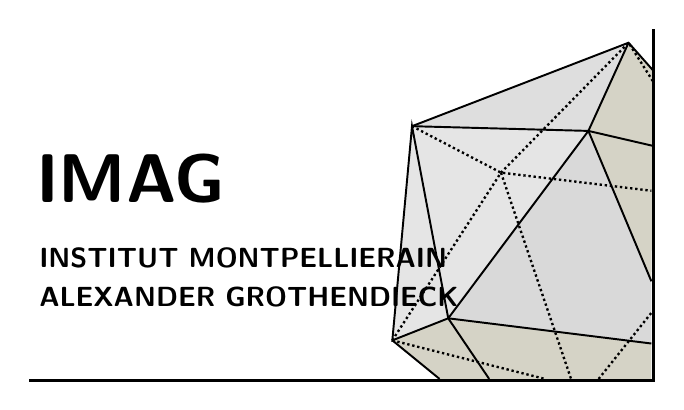
\begin{tikzpicture}[x=1cm,y=-1cm]
\fill[black!13] (4.96,1.38)--(7.71,.32)--(7.20,1.44)--cycle;
\fill[black!10] (4.96,1.38)--(7.20,1.44)--(5.42,3.82)--(4.71,4.10)--cycle;
\fill[black!15] (7.20,1.44)--(8.00,3.35)--(8.00,4.14)--(5.42,3.82)--cycle;
\fill[yellow!15!gray!45] (7.71,.32)--(8.02,.67)--(8.02,1.63)--(7.20,1.44)--cycle;
\fill[yellow!15!gray!45] (7.20,1.44)--(8.02,1.63)--(8.00,3.35)--cycle;
\fill[yellow!15!gray!45] (4.71,4.10)--(5.42,3.82)--(8.00,4.14)--(8.00,4.59)--(5.31,4.59)--cycle;
\draw[line width=.7pt] (4.96,1.38)--(7.71,.32)--(8.02,.67);
\draw[line width=.7pt] (4.96,1.38)--(7.20,1.44)--(8.02,1.63);
\draw[line width=.7pt] (7.71,.32)--(7.20,1.44)--(5.42,3.82)--(4.71,4.10)--(4.96,1.38)--(5.42,3.82)--(5.94,4.59);
\draw[line width=.7pt] (4.71,4.10)--(5.31,4.59);
\draw[line width=.7pt] (5.42,3.82)--(8.00,4.14);
\draw[line width=.7pt] (7.20,1.44)--(8.00,3.35);
\draw[densely dotted,line width=.85pt] (4.96,1.38)--(6.09,1.97)--(8.00,2.20);
\draw[densely dotted,line width=.85pt] (4.71,4.10)--(6.09,1.97)--(7.71,.32)--(8.02,.81);
\draw[densely dotted,line width=.85pt] (6.09,1.97)--(6.98,4.59);
\draw[densely dotted,line width=.85pt] (4.71,4.10)--(6.65,4.59);
\draw[densely dotted,line width=.85pt] (7.33,4.59)--(8.00,3.75);
\draw[line width=1.2pt] (.10,4.61)--(8.03,4.61)--(8.03,.15);
\node[anchor=west,inner sep=0,font=\sffamily\bfseries\fontsize{48}{50}\selectfont] at (.18,2.05) {IMAG};
\node[anchor=west,inner sep=0,font=\sffamily\bfseries\fontsize{10}{12}\selectfont] at (.22,3.05) {INSTITUT MONTPELLIERAIN};
\node[anchor=west,inner sep=0,font=\sffamily\bfseries\fontsize{10}{12}\selectfont] at (.22,3.55) {ALEXANDER GROTHENDIECK};
\end{tikzpicture}}
\scanpage{2}

Structures stratifiées

\diagram{\begin{tabular}{r p{.72\linewidth} r}
1.&La situation type -- préliminaires d'un programme.&1.\\[1em]
2.&Stratifications globales: le formalisme $\frac12$ simplicial (sans tubes)&10\\[1em]
3.&\deleted{\unsure{Strat}} Introduction des tubes&16\\[1em]
4.&Topos canoniques associés à une stratification (globale)&23
\end{tabular}}
\margin{1}
\scanpage{3}

\diagram{\begin{tikzcd}[ampersand replacement=\&,column sep=large,row sep=small]
E_0\arrow[r,bend left=50,"\delta_0"]\&E_1\arrow[l,shift right=1.2ex,"p_0"']\arrow[l,shift left=1.2ex,"p_1"]\arrow[r,bend left=50,"{\delta_1,\delta_2,\delta_3}"]\arrow[r,bend left=60]\arrow[r,bend left=70]\&E_2\arrow[l,shift right=2.2ex,"p_{12}"']\arrow[l,"\unsure{p_{23}}"']\arrow[l,shift left=2.2ex,"p_{13}"]\\
\&\unsure{\mathfrak S_2|\mathcal G_2}\arrow[d,phantom,"\ni" rotate=90]\&\unsure{\mathfrak S_3|\mathcal G_3}\arrow[d,phantom,"\ni" rotate=90]\\
\&\sigma\&\overbrace{\rho,\sigma_1,\sigma_2,\sigma_3}\\
\&\&\rho^2
\end{tikzcd}}
\deleted{\diagram{\begin{tikzcd}[ampersand replacement=\&,column sep=large]
{}\arrow[r,bend right=40,"\unsure{\delta_1}"']\arrow[r,bend right=55,"\unsure{\delta_2}"']\arrow[r,bend right=70,"\delta_3"']\&{}
\end{tikzcd}}}
\[\boxed{\begin{aligned}
\delta_{\unsure{3|2}}(x,y)&=(x,x,y)\\
\delta_1(x,y)&=(y,x,x)\\
\delta_2(x,y)&=(x,y,x)
\end{aligned}}\]
\margin{\deleted{$\delta_1\sigma(x,y)=(y,y,x)$}\quad $\unsure{=}$\\$\sigma_3\delta_3$}
\mspage{\textcircled{1}}
\[p_1=p_0\sigma,\quad p_0=p_1\sigma\]
\[\boxed{\begin{aligned}
p_{12}(x,y,z)&=(x,y)\\
p_{\deleted{\unsure{21}}\inserted{23}}(x,y,z)&=(y,z)\\
p_{31}(x,y,z)&=(z,x)
\end{aligned}}\]
\margin{$\rho(x,y,z)=(y,z,x)$}
\deleted{\[\unsure{p_{12}=p_{23}}\]}
\[\boxed{\left\{\begin{aligned}
p_{23}&=p_{12}\rho\\
p_{31}&=p_{23}\rho=p_{12}\rho^2\\
p_{12}&=p_{31}\rho=p_{23}\rho^2
\end{aligned}\right.}\]
\[\begin{aligned}
\sigma p_{12}&=p_{12}\sigma_3\\
\sigma p_{23}&=p_{23}\sigma_1\\
\sigma p_{31}&=p_{31}\sigma_2
\end{aligned}\]
\deleted{\[(x,y,z)\quad(y,z,x)\quad(y,x,z)\]}
\[\left\{\begin{aligned}
\delta_1&=\rho\delta_2=\rho^2\delta_3\\
\delta_2&=\rho\delta_3=\rho^2\delta_1\\
\delta_3&=\rho\delta_1=\rho^2\delta_2\unsure{\,a}
\end{aligned}\right.\]

\deleted{\unsure{a}} Il suffit de \unsure{avoir} $p_0,p_{12},\delta_0,\delta_1$ entre les trois ensembles $E_0$, $(E_1,\unsure{\mathfrak S_2|\mathcal G_2})$, $(E_2,\unsure{\mathfrak S_3|\mathcal G_3})$, avec les relations
\[\boxed{p_0\delta_0=\mathrm{id}_{E_0}},\quad\deleted{\unsure{p_1\delta_0}}\]
\[\delta_0p_0=p_{12}\underbrace{\delta_3}_{\rho\deleted{\unsure{\sigma}}\delta_1}=\underbrace{p_{23}}_{p_{12}\rho}\underbrace{\delta_1}_{\deleted{\unsure{\rho}}}=\underbrace{p_{31}}_{p_{12}\rho^2}\underbrace{\delta_2}_{\rho^2\delta_1}\]
\[\boxed{\sigma\delta_0=\delta_0}\]
\deleted{\[\text{i.e.}\quad\underbrace{\delta_0p_0}=\underbrace{p_{12}\delta_1}_{\sigma}=\underbrace{p_{12}\rho\delta_1}_{\mathrm{id}}=\underbrace{p_{12}\rho^2\delta_1}\]}
\deleted{\[\underbrace{(p_{12}\rho)}_{p_{23}}\delta_1\overset{??}{\ne}p_{12}(\underbrace{\rho\delta_1}_{\delta_3})\]}
\[\boxed{\begin{aligned}
\delta_0p_0&=p_{12}\overbrace{\rho\delta_1}^{\delta_3}\\
\mathrm{id}_{E_1}&=p_{12}\underbrace{\rho^2\delta_1}_{\delta_2}\\
\sigma&=p_{12}\delta_1
\end{aligned}}\]
\margin{$\boxed{\sigma_{\unsure{3|1}}\delta_1=\delta_1}$\\$\boxed{p_{12}\sigma_3=\sigma p_{12}}$}
\deleted{$\unsure{\mathrm{ens}}$}
\diagram{\begin{tikzcd}[ampersand replacement=\&,column sep=large,row sep=small,execute at end picture={\draw (current bounding box.south west) rectangle (current bounding box.north east);}]
\deleted{\unsure{\mathfrak S_1}}\&\unsure{\mathfrak S_2|\mathcal G_2}\&\unsure{\mathfrak S_3|\mathcal G_3}\\
E_0\arrow[r,bend right=30,"\delta_0"']\&E_1\arrow[l,"p_0"']\arrow[r,bend right=30,"\delta_1"']\&E_2\arrow[l,"p_{12}"']
\end{tikzcd}}
\[\boxed{\rho\delta_1\delta_0=\sigma_1\delta_1\delta_0=\delta_1\delta_0}\]
\[\underbrace{p_0p_{12}}_{p_{\unsure{1|2}}}=p_0\overbrace{\underbrace{p_{12}\deleted{\unsure{\sigma}}\rho^2}_{p_{31}}\sigma_2}^{p_{12}}\]
\margin{2}
\scanpage{4}

\hrule
\begin{tabular}{p{.47\linewidth}p{.47\linewidth}}
\textbf{ACADEMIE D'AIX-MARSEILLE} & AVIGNON le 6 décembre 1990\\
\rule{3cm}{.4pt}&\\
\textbf{INSPECTION ACADEMIQUE} & Jacques ROUX, responsable\\
\textbf{DE VAUCLUSE}&départemental de l'Action\\
\rule{1cm}{.4pt}&Culturelle,\\[1em]
C.D.A.C.N°16&à\\[1em]
&M
\end{tabular}

\uline{OBJET} : Projets d'Action Educative Collège\\
Année scolaire 1990/1991

L'attribution des aides aux P.A.E. se déroulera cette année en deux temps :

\begin{tabular}{l p{.72\linewidth}}
DECEMBRE & - instruction des dossiers\\
&par l'Inspection Académique\\[1em]
&propositions à la M.I.A.D.A.C.\\[1em]
JANVIER & - Monsieur le Recteur attribue\\
&une aide globalisée à Monsieur\\
&l'Inspecteur d'Académie.
\end{tabular}

Une commission se réunit vers le 15 janvier 1991, afin d'assurer la ventilation des aides au niveau du département. Je vous demanderai alors de participer à cette Commission.

P/L'Inspecteur d'Académie

\unsure{Roux}
\unsure{ROUX}
\margin{3}
\scanpage{5}

\deleted{\[\begin{array}{ccc}
p_0/p_1&p_{12}\quad p_{23}\quad p_{31}&\delta_1\quad\delta_2\quad\delta_3\\
\delta_0&\deleted{\unsure{\sigma p_{12}\quad\sigma p}}&\\
&p_{21}\quad p_{32}\quad p_{13}&
\end{array}\]}
\mspage{\textcircled{2}}
\[\deleted{\delta_0p_0,\delta_0p_1,}\quad\mathrm{id},\sigma\]
\diagram{\begin{tikzcd}[ampersand replacement=\&,column sep=large,row sep=small,execute at end picture={\draw (current bounding box.south west) rectangle (current bounding box.north east);}]
\&\unsure{\mathfrak S_2|\mathcal G_2}\&\unsure{\mathfrak S_3|\mathcal G_3}\\
E_0\arrow[r,shift right=1.3ex,"\delta_0"']\&E_1\arrow[l,shift right=1.3ex,"p_0"']\arrow[r,bend right=25,"\delta_1"']\&E_2\arrow[l,"p_{12}"']
\end{tikzcd}}
\deleted{\[\delta_1p_{12}\]}
\[\boxed{\begin{aligned}p_0\delta_0&=\mathrm{id}_{E_0}\\\sigma\delta_0&=\delta_0\end{aligned}}\]
\[\boxed{\begin{aligned}
p_{12}\delta_1&=\sigma\qquad\text{(involution}\\
p_{12}\overset{\deleted{\unsure{\mathrm{id}}}}{\underbrace{\rho\delta_1}_{\delta_3}}&=\delta_0p_0\qquad\text{(idempotent)}\\
p_{12}(\underbrace{\rho^2\delta_1}_{\delta_2})&=\mathrm{id}
\end{aligned}}\]
\margin{$\boxed{\deleted{p_0,p_1}}$\\\diagram{\begin{tikzcd}[execute at end picture={\foreach \ovalnode in {ovalp}{\begingroup\pgfextractx{\dimen0}{\pgfpointdiff{\pgfpointanchor{\ovalnode}{west}}{\pgfpointanchor{\ovalnode}{east}}}\pgfextracty{\dimen2}{\pgfpointdiff{\pgfpointanchor{\ovalnode}{south}}{\pgfpointanchor{\ovalnode}{north}}}\dimen0=.7071067812\dimen0\dimen2=.7071067812\dimen2\draw (\ovalnode.center) ellipse[x radius=\the\dimen0,y radius=\the\dimen2];\endgroup}}]|[alias=ovalp,rectangle,draw=none]|p_0,p_1\end{tikzcd}}}
\diagram{\begin{tikzcd}[ampersand replacement=\&,column sep=large,row sep=small,execute at end picture={\foreach \ovalnode in {ovald,ovaldp,ovalpp}{\begingroup\pgfextractx{\dimen0}{\pgfpointdiff{\pgfpointanchor{\ovalnode}{west}}{\pgfpointanchor{\ovalnode}{east}}}\pgfextracty{\dimen2}{\pgfpointdiff{\pgfpointanchor{\ovalnode}{south}}{\pgfpointanchor{\ovalnode}{north}}}\dimen0=.7071067812\dimen0\dimen2=.7071067812\dimen2\draw (\ovalnode.center) ellipse[x radius=\the\dimen0,y radius=\the\dimen2];\endgroup}}]
\boxed{\begin{gathered}\sigma_1\delta_1=\delta_1\\p_{12}\sigma_3=\underbrace{\sigma p_{12}}_{p_{21}}\end{gathered}}\&|[alias=ovald,rectangle,draw=none]|\delta_1,\delta_2,\delta_3\arrow[l,bend right=15,shorten <=1em]\&|[alias=ovaldp,rectangle,draw=none]|\begin{gathered}\delta'_1=\delta_1\sigma\\\delta'_2=\delta_2\sigma\\\delta'_3=\delta_3\sigma\end{gathered}\\
\&|[alias=ovalpp,rectangle,draw=none]|\begin{gathered}p_{12},p_{23},p_{31},\unsure{{}^3}\\p_{21},p_{32},p_{13}\end{gathered}\&
\end{tikzcd}}
\[\boxed{\begin{gathered}
\rho(\delta_1\delta_0)=\sigma_1(\delta_1\delta_0)=\delta_1\delta_0\\
\text{i.e.}\qquad g(\delta_1\delta_0)=\delta_1\delta_0\quad\text{pour }g\in\unsure{\mathfrak S_3|\mathcal G_3}
\end{gathered}}\]
\[\boxed{p_0p_{12}\sigma_{\unsure{1}}=\underbrace{p_0p_{12}}_{q_1}}\]
\margin{\diagram{\begin{tikzcd}[execute at end picture={\foreach \ovalnode in {ovalq}{\begingroup\pgfextractx{\dimen0}{\pgfpointdiff{\pgfpointanchor{\ovalnode}{west}}{\pgfpointanchor{\ovalnode}{east}}}\pgfextracty{\dimen2}{\pgfpointdiff{\pgfpointanchor{\ovalnode}{south}}{\pgfpointanchor{\ovalnode}{north}}}\dimen0=.7071067812\dimen0\dimen2=.7071067812\dimen2\draw (\ovalnode.center) ellipse[x radius=\the\dimen0,y radius=\the\dimen2];\endgroup}}]|[alias=ovalq,rectangle,draw=none]|q_1,q_2,q_3\end{tikzcd}}}
\margin{4}
\scanpage{6}

\hrule
\begin{tabular}{p{.47\linewidth}p{.47\linewidth}}
\textbf{ACADEMIE D'AIX-MARSEILLE} & AVIGNON le 6 décembre 1990\\
\rule{3cm}{.4pt}&\\
\textbf{INSPECTION ACADEMIQUE} & Jacques ROUX, responsable\\
\textbf{DE VAUCLUSE}&départemental de l'Action\\
\rule{1cm}{.4pt}&Culturelle,\\[1em]
C.D.A.C.N°16&à\\[1em]
&M
\end{tabular}

\uline{OBJET} : Projets d'Action Educative Collège\\
Année scolaire 1990/1991

L'attribution des aides aux P.A.E. se déroulera cette année en deux temps :

\begin{tabular}{l p{.72\linewidth}}
DECEMBRE & - instruction des dossiers\\
&par l'Inspection Académique\\[1em]
&propositions à la M.I.A.D.A.C.\\[1em]
JANVIER & - Monsieur le Recteur attribue\\
&une aide globalisée à Monsieur\\
&l'Inspecteur d'Académie.
\end{tabular}

Une commission se réunit vers le 15 janvier 1991, afin d'assurer la ventilation des aides au niveau du département. Je vous demanderai alors de participer à cette Commission.

P/L'Inspecteur d'Académie

\unsure{Roux}
\unsure{ROUX}
\margin{5}
\scanpage{7}
\mspage{\textcircled{3}}

\deleted{\[p_0p_{12}=p_0p_{13}=p_0\underbrace{p_{12}\rho^2}_{p_{31}}\sigma_2\]}
\deleted{\[\rho^2\sigma_2=\sigma_3\rho^2\]}
\deleted{\diagram{\begin{tikzcd}[ampersand replacement=\&,row sep=small]
(x,y,z)\arrow[r,mapsto]\&(z,y,x)\\
{}\arrow[r]\&(x,z)\arrow[r]\&x
\end{tikzcd}}}
\deleted{\[p_0p_{12}\sigma_1=p_0p_{12}\]}
\deleted{\[(x,x,y)\]}
\deleted{\[\rho^2\sigma_2:\quad(x,y,z)\mapsto(z,y,x))\qquad\mapsto(\uline{y,x},z)\]}
\deleted{\[\delta_1\sigma=(x,y,y)\qquad z,x,y\]}
\deleted{\[(x,x,y)\qquad(y,y,x)\]}
\deleted{\[(x,y,z)\mapsto(z,x,y)\qquad(x,z,y)=\sigma_1\]}

\mspage{\textcircled{3}}
Si $E_0$ est réduit à un pt, les $E_1,E_2$ deviennent des ens. pointés, et $\unsure{\mathfrak S_2|\mathcal G_2},\unsure{\mathfrak S_3|\mathcal G_3}$ respectent \unsure{la ponctuation|les ponctuations}.
\margin{par $\delta_0,\delta_1\delta_0$}
\margin{(\unsure{``ponctués''})}
\deleted{On a.}
\deleted{\unsure{qui respecte les}}
\unsure{Ainsi|Alors}, en plus des opérations de $\unsure{\mathfrak S_2|\mathcal G_2},\unsure{\mathfrak S_3|\mathcal G_3}$, on a
\diagram{\begin{tikzcd}[ampersand replacement=\&,column sep=large]E_1\arrow[r,bend right=35,"\delta_1"']\&E_2\arrow[l,"p_{12}"']\end{tikzcd}}
, où $\delta_1$ \inserted{et $p_{12}$} respectent les ponctuations, et où $p_{12},\delta_1$ satisfont aux cinq relations supplémentaires
\[\boxed{\begin{aligned}
p_{12}\delta_1&=\sigma\\
p_{12}\underbrace{\rho\delta_1}_{\delta_3}&=\text{application constante de valeur }e_1\quad\text{(pt marqué de }E_1\text{)}\\
p_{12}\underbrace{\rho^2\delta_1}_{\delta_2}&=\mathrm{id}_{E_1}\\
\sigma_1\delta_1&=\delta_1\\
p_{12}\sigma_3&=\sigma p_{12}
\end{aligned}}\]
\margin{$\boxed{\begin{aligned}
p_{12}\delta_2&=\mathrm{id}_{E_1}\\
p_{12}\underbrace{\rho\delta_2}_{\delta_1}&=\sigma\\
p_{12}\underbrace{\rho^2\delta_2}_{\delta_3}&=e_1\quad\text{(application de }E_1\text{ sur }e_1\text{)}
\end{aligned}}$}
\margin{$\uline{p_{12}\sigma_3=\sigma p_{12}}$\\$\sigma_2\delta_2=\delta_2$\\\deleted{$\unsure{p_{12}\sigma_3=\sigma p_{12}}$}\\\deleted{$\unsure{\mathrm{id}}$}\\\diagram{\begin{tikzcd}[ampersand replacement=\&,column sep=large]E_1\arrow[r,bend right=25,"\delta_1"']\&E_2\arrow[l,"p_{12}"']\end{tikzcd}}}
\margin{6}
\scanpage{8}

\hrule
\begin{tabular}{p{.47\linewidth}p{.47\linewidth}}
\textbf{ACADEMIE D'AIX-MARSEILLE} & AVIGNON le 6 décembre 1990\\
\rule{3cm}{.4pt}&\\
\textbf{INSPECTION ACADEMIQUE} & Jacques ROUX, responsable\\
\textbf{DE VAUCLUSE}&départemental de l'Action\\
\rule{1cm}{.4pt}&Culturelle,\\[1em]
C.D.A.C.N°16&à\\[1em]
&M
\end{tabular}

\uline{OBJET} : Projets d'Action Educative Collège\\
Année scolaire 1990/1991

L'attribution des aides aux P.A.E. se déroulera cette année en deux temps :

\begin{tabular}{l p{.72\linewidth}}
DECEMBRE & - instruction des dossiers\\
&par l'Inspection Académique\\[1em]
&propositions à la M.I.A.D.A.C.\\[1em]
JANVIER & - Monsieur le Recteur attribue\\
&une aide globalisée à Monsieur\\
&l'Inspecteur d'Académie.
\end{tabular}

Une commission se réunit vers le 15 janvier 1991, afin d'assurer la ventilation des aides au niveau du département. Je vous demanderai alors de participer à cette Commission.

P/L'Inspecteur d'Académie

\unsure{Roux}
\unsure{ROUX}
\margin{7}
\scanpage{9}

\textbf{ACADEMIE D'AIX-MARSEILLE}\\
\rule{3cm}{.4pt}\\
\textbf{INSPECTION ACADEMIQUE}\\
\textbf{DE VAUCLUSE}\\
\rule{1cm}{.4pt}
\mspage{\textcircled{4}}
\[\begin{aligned}
p_{12}\delta_1(x)&=\sigma(x)\\
\underbrace{p_{12}\rho}_{p_{23}}\delta_1(x)&=\delta_0p_0(x)\\
\underbrace{p_{12}\rho^2}_{p_{31}}\delta_1(x)&=x
\end{aligned}\]
\margin{NB $\delta_1(x)$ ne peut être \unsure{fixe|fixé} par $\rho$ (donc par $\unsure{\mathfrak S_3|\mathcal G_3}$) que si $x=\delta_0p_0(x)$ (condition néc. et suff.)}
\[\boxed{\begin{gathered}
\delta_0p_0(x)=1\\
\sigma(x)x=1\\[.5em]
p_{12}(z)p_{23}(z)p_{31}(z)=1
\end{gathered}}\]
\[\sigma(x)\underbrace{\delta_0p_0(x)}_{\substack{\Vert\\1}}x=1\]
pour $z\in E_2$ (une relation \deleted{\unsure{par}} supplémentaire par orbite \inserted{sous $\unsure{\mathfrak S_3|\mathcal G_3}$} qui ne rencontre pas $\delta_1(E_1)$)
\diagram{\begin{tikzcd}[ampersand replacement=\&,column sep=large,row sep=large]
\delta_1\&F\times F\times F\arrow[loop above,"\sigma_1"]\arrow[d,shift right=1.2ex,"p_{12}"']\arrow[d,shift left=1.2ex,"p_{13}"]\arrow[rr,no head]\arrow[rr,shift right=1.5ex,no head]\&\&{}\\
F_\alpha\arrow[r,hook,no head]\&F\times F\arrow[d,"\mathrm{pr}_0"]\&\&\alpha\in E_1\\
\&F\&\&
\end{tikzcd}}
\[(x,y)\mapsto y\]
\[(x,y)\times_{\unsure{x}}(x',y')\sim(x,\deleted{y},y')\]
\[E_2(\alpha)\ni\delta_1(\alpha)=\delta_1\sigma(\alpha)\]
\[\pi_0(F_\alpha\times_F F_\alpha)=\overbrace{p_{12}^{-1}(\alpha)\cap p_{13}^{-1}(\alpha)}\qquad\text{stable par }\sigma_1\]
\margin{Le petit coq aux \unsure{champs}\\\deleted{\unsure{tél}}\\$\boxed{32\ 41\ 04\ 19}$}
\margin{$y,x,y$}
Prenons $\alpha\ne\delta_1$, alors $\delta_2\notin p_{12}^{-1}(\alpha)$

les pts fixes par $\sigma_1$ sont dans image $\delta_1(E_1)$, mais $p_{12}(\delta_1(x))=p_{13}(\delta_1(x))=\sigma x$, donc \deleted{\unsure{il faut}}
\deleted{\unsure{faut} $\sigma x={}$} $\delta_1(x)\in E_2(\alpha)\Longleftrightarrow\sigma x=\alpha$ i.e. $x=\uline{\sigma\alpha}$

et $\uline{\delta_1\sigma}(\alpha)$ joue le rôle de $\delta_{\unsure{2|1}}=\delta_1(\alpha)$
\margin{8}
\scanpage{11}
\mspage{1}

Hyperrecouvrements.

Soit $\mathcal X$ une catégorie $\mathcal U$-topos. On veut définir \deleted{\unsure{une}} la notion d'\uline{hyperrecouvrement} de $\mathcal X$ (ou encore, du topos défini par $\mathcal X$), indexé par une petite catégorie $A$. \deleted{Un tel hyp} Ce sera par définition un foncteur
\diagram{\begin{tikzcd}[ampersand replacement=\&,row sep=small]
\varphi:\quad A\arrow[r]\&\mathcal X\\
\alpha\arrow[r,mapsto]\&U_\alpha\ (=\varphi(\alpha))
\end{tikzcd}}
, satisfaisant certaines conditions, inspirées par la \unsure{coho} \inserted{``\unsure{Cechiste}''} des recouvrements et de leurs nerfs, et le raffinement de ce \unsure{p.d.v.|p.d.} suggéré par Cartan (pour les espaces topologiques non paracompacts). Voici les conditions qui me viennent à l'esprit:

\uline{Hyp 1} Les objets $U_\alpha$ ($\alpha\in\mathrm{Ob}\,A$) recouvrent l'objet final $e_{\mathcal X}$ de $\mathcal X$.

\deleted{\uline{Hyp 1'} Pour tout $\alpha_0\in\mathrm{Ob}\,A$, le foncteur
\[A/\alpha_0\longrightarrow\mathcal X/U_{\alpha_0}\]
satisfait à Hyp 1, l'ens. des flèches $U_\alpha\longrightarrow U_{\alpha_0}$, associé aux flèches $\alpha\longrightarrow\alpha_0$ de but $\alpha_0$ dans $A$,}
\margin{Est satisfait tautologiquement!}
\margin{10}
\scanpage{12}
\mspage{2}

est couvrant.

\uline{Hyp 2}\unsure{a} Pour $\alpha,\beta\in\mathrm{Ob}\,A$, l'ens des \deleted{flèches} diagrammes
\diagram{\begin{tikzcd}[ampersand replacement=\&,column sep=small,row sep=small]\&\alpha\\\gamma\arrow[ur]\arrow[dr]\&\\\&\beta\end{tikzcd}}
dans $A$ (i.e. l'ens. des objets de $A_{/\alpha\times\beta}$, où $\alpha\times\beta$ est le produit cartésien dans $\widehat A$), indexant les flèches correspondantes $U_\gamma\longrightarrow U_\alpha\times U_\beta$, donne une famille couvrant $U_\alpha\times U_\beta$.

[Idem pour une suite finie \inserted{(non vide)} $\alpha_0,\alpha_1,\ldots,\alpha_n$ ($n\in\mathbb N^{\deleted{\unsure{*}}}$) d'objets de $A$, et les \deleted{diagr.} flèches
\[U_\gamma\longrightarrow U_{\alpha_0}\times U_{\alpha_1}\times\cdots\times U_{\alpha_n}\]
indexées par les objets de $A_{/\alpha_0\times\alpha_1\times\cdots\alpha_n}$.]
\margin{[Hyp. 2 généralisé]}

Pour $n=0$, on retrouve Hyp 1', pour $n=1$, la formulation initiale de Hyp 2. Mais Hyp 2 pour $n=1$ implique-t-il Hyp 2 pour \deleted{$\unsure{n>1}$ \unsure{quelconque}} $n\geq1$. On voit qu'il en est ainsi, par récurrence, en utilisant le fait que la famille composée de deux familles couvrantes
\diagram{\begin{tikzcd}[ampersand replacement=\&,column sep=large]
U_{\gamma'}\arrow[r,"\varphi(v)"]\&U_\gamma\times U_{\alpha_{n+1}}\arrow[r,"\varphi(u)\times\mathrm{id}_{U_{\alpha_{n+1}}}"]\&(U_{\alpha_0}\times\cdots\times U_{\alpha_n})\times U_{\alpha_{n+1}}
\end{tikzcd}}
($v$ parcourant les flèches $\gamma'\longrightarrow\gamma\times\alpha_{n+1}$, et $u$ les flèches $\gamma\longrightarrow\alpha_0\times\cdots\times\alpha_n$) est couvrante. Ainsi Hyp 1' \deleted{implique} \inserted{$+$} Hyp 2\unsure{a}
\margin{11}
\scanpage{13}
\mspage{3}

forme initiale (cas $\alpha,\beta$) implique Hyp. 2 sous sa forme générale (en termes de $\alpha_0,\alpha_1,\ldots,\alpha_n$).

\uline{Hyp. 2'}: Pour tout $\alpha_0\in\mathrm{Ob}\,A$, le foncteur induit $A_{/\alpha_0}\longrightarrow\mathcal X_{/\alpha_0}$ satisfait à Hyp 2 i.e. pour tout diagramme
\diagram{\begin{tikzcd}[ampersand replacement=\&,column sep=small,row sep=small]\alpha_1\arrow[dr]\&\&\alpha_2\arrow[dl]\\\&\alpha_0\&\end{tikzcd}}
, regardant les carrés commutatifs de $A$ qui le complètent en
\diagram{\begin{tikzcd}[ampersand replacement=\&,column sep=small,row sep=small]
\&\gamma\arrow[dl]\arrow[dr]\&\\
\alpha_1\arrow[dr]\&\&\alpha_2\arrow[dl]\\
\&\alpha_0\&
\end{tikzcd}}
, i.e. les objets de $A_{/\alpha_1\times_{\alpha_0}\alpha_2}$, la famille des flèches correspondantes
\[U_\gamma\longrightarrow U_{\alpha_1}\times_{U_{\alpha_0}}U_{\alpha_2}\]
est couvrante (i.e., épimorphique).

Les hypothèses Hyp 1, 2, 2' se reformulent joliment, en termes du prolongement canonique
\[\varphi_!:\widehat A\longrightarrow\mathcal X\]
de $\varphi$ en un foncteur \inserted{$\widehat A\longrightarrow\mathcal X$} commutant \deleted{\unsure{à}} aux petites $\lim_{\longrightarrow}$. Ce sont respectivement
\margin{12}
\scanpage{14}
\mspage{4}

\[
\text{a)}\quad \varphi_!(e_{\widehat A})\longrightarrow e_{\mathcal X}\quad\text{est épi}
\]
\[
\text{b)}\quad \varphi_!(\alpha\times\beta)\longrightarrow
\varphi_!(\alpha)\times\varphi_!(\beta)\quad\text{est épi}
\qquad \forall\alpha,\beta\text{ dans }\operatorname{Ob}A
\]
\[
\text{c)}\quad \varphi_!(\alpha\times_{\alpha_0}\beta)\longrightarrow
\varphi_!(\alpha)\times_{\varphi_!(\alpha_0)}\varphi_!(\beta)\quad\text{est épi}
\]
$\forall$ diagramme
\diagram{\begin{tikzcd}[ampersand replacement=\&,column sep=small,row sep=small]
\alpha\arrow[dr]\&\&\beta\arrow[dl]\\
\&\alpha_0\&
\end{tikzcd}}
dans $A$.

Un cas particulièrement agréable où ces conditions sont satisfaites, c'est quand $\varphi_!$ est exact à gauche, i.e. qu'il correspond \deleted{\unsure{à}} à un morphisme de topos
\[
f:\mathcal X\longrightarrow\widehat A
\]
par la formule
\[
\varphi_!=f^*.
\]
Alors dans a) b) c) les flèches épi en question sont même des iso, et je présume que l'inverse est vrai également. Oui -- et c'est essentiellement évident, en écrivant canoniquement, pour un $F\in\operatorname{Ob}\widehat A$, $F=\varinjlim_{A/F}\alpha$ \unsure{$\ldots$}. On voit

\deleted{Mais peut-on avoir}

de la $=$ façon que b) et c)

\margin{13}
\scanpage{15}
\mspage{5}

impliquent
\[
\text{b')}\quad\varphi_!(F\times G)\longrightarrow\varphi_!(F)\times\varphi_!(G)\quad\text{épi}
\qquad\forall F,G\text{ dans }\operatorname{Ob}\widehat A
\]
\[
\text{c')}\quad\varphi_!(G\times_F H)\longrightarrow
\varphi_!(G)\times_{\varphi_!(F)}\varphi_!(H)\quad\text{épi}
\]
$\forall$ diagramme
\diagram{\begin{tikzcd}[ampersand replacement=\&,column sep=small,row sep=small]
G\arrow[dr]\&\&H\arrow[dl]\\
\&F\&
\end{tikzcd}}
dans $\widehat A$.

et de là, plus généralement, la forme équivalente \unsure{unique} de Hyp 1, 2, 2' :

\figure{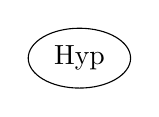
\begin{tikzpicture}\draw (0,0) ellipse (.65 and .38);\node at (0,0) {Hyp};\end{tikzpicture}}
Pour tout diagramme fini $(F_i)_{i\in I}$ dans $\widehat A$, la flèche canonique
\[
\varphi_!\left(\varprojlim_I F_i\right)\longrightarrow\varprojlim_I\varphi_!(F_i)
\]
est épi.

(Il suffit d'ailleurs de le postuler quand les $F_i$ sont dans $A$, et dans les trois cas particuliers $I=\bullet$, $\bullet\ \bullet$,
\diagram{\begin{tikzcd}[ampersand replacement=\&,column sep=tiny,row sep=tiny]
\bullet\arrow[dr]\&\&\bullet\arrow[dl]\\
\&\bullet\&
\end{tikzcd}}, correspondants aux axiomes Hyp 1, Hyp 2, Hyp $\unsure{1|2}'$.)

Mais cette hypothèse peut-elle être vérifiée, sans que $\varphi_!$ soit $=$ ex. à gauche ?

\margin{14}
\scanpage{17}
\mspage{\textcircled{1}}

\diagram{\begin{tikzcd}[ampersand replacement=\&]
\mathbb E_n\arrow[r,shift left,"\delta_n"]\&\mathbb E_{n+1}\arrow[l,shift left,"K_n"]
\end{tikzcd}}
$n\in\mathbb N^*\quad\text{i.e. }n\geq1$

\[
\left.\begin{aligned}
\delta_n &: [1,n]\hookrightarrow[1,n+1]&&\text{inclusion}\\
K_n &: [1,n]\longleftarrow[1,n+1]&&\text{rétraction}
\end{aligned}\right]
\]
\margin{$\unsure{\mathfrak S_n|\mathcal G_n}$ opère sur $\mathbb E_n$
\diagram{\begin{tikzcd}[ampersand replacement=\&]
\unsure{\mathfrak S_n|\mathcal G_n}\arrow[r,hook,"i_n"]\&\unsure{\mathfrak S_{n+1}|\mathcal G_{n+1}}
\end{tikzcd}}}

\margin{$\delta_nK_n\overset{\mathrm{def}}=\rho_{n+1}$ (projection dans $\mathbb E_{n+1}$, rétraction sur $\mathbb E_n\subset\mathbb E_{n+1}$)}
\[
\boxed{\left\{\begin{aligned}
K_n\delta_n&=\mathrm{id}_{\mathbb E_n}\\
\delta_n\sigma&=i_n(\sigma)\delta_n&&\text{si }\sigma\in\unsure{\mathfrak S_n|\mathcal G_n}\quad\text{pour }n\geq2\\
\sigma K_n&=K_n i'_n(\sigma)&&\text{si }\sigma\in\unsure{\mathfrak S_{n-1}|\mathcal G_{n-1}}\quad\text{pour }n\geq3\\
K_n\sigma_{n+1}&=K_n
\end{aligned}\right.}
\]
\margin{où $i'_n=i_n i_{n-1}:\unsure{\mathfrak S_{n-1}|\mathcal G_{n-1}}\longrightarrow\unsure{\mathfrak S_n|\mathcal G_n}\longrightarrow\unsure{\mathfrak S_{n+1}|\mathcal G_{n+1}}$}
\margin{où $\sigma_m\in\unsure{\mathfrak S_m|\mathcal G_m}$ est la transposition $(m-1,m)$}

\diagram{\begin{tikzcd}[ampersand replacement=\&]
\mathbb E_n^*\arrow[r,shift right=2,"d_n=K_n^*"']\&\mathbb E_{n+1}^*\arrow[l,shift right=2,"p_n=\delta_n^*"']
\end{tikzcd}}

\[
(*)\quad\boxed{\begin{aligned}
\delta_n^*K_n^*&=\mathrm{id}_{E_n^*}\\
\sigma\delta_n^*&=\delta_n^*i_n(\sigma)\qquad(\sigma\in\unsure{\mathfrak S_n|\mathcal G_n})\\
K_n^*\sigma_{\unsure{n}}&=i'_n(\sigma)K_n^*\qquad\text{(\unsure{''|id})}\\
\sigma_{n+1}K_n^*&=K_n^*
\end{aligned}}
\]
réalisation dans $(\mathrm{Ens})$ de syst. de
$(\underbrace{E_n^*}_{\unsure{\mathfrak S_n|\mathcal G_n}\text{-ens.}},\delta_n^*,K_n^*)$
satisfaisant aux relations $(*)$, \uline{plus}

\[
(**)\quad\boxed{
\underbrace{E_{p+q}^*\longrightarrow E_p^*\times E_q^*}_{\vphantom{A}}
\quad\text{surjectif pour }p,q\geq1}
\]
\inserted{$(\alpha^*_{\deleted{\unsure{p+q}}p+q,p},\beta^*_{\deleted{\unsure{p+q}}p+q,q})$}

où
\[
\alpha^*_{n,p}:E_n^*\longrightarrow E_p^*\qquad(n>p\geq1)
\]
défini par
\[
\boxed{\alpha^*_{n,p}=\delta_p^*\delta_{p+1}^*\cdots\delta_{n-1}^*}
\]
\diagram{\begin{tikzcd}[ampersand replacement=\&,column sep=small]
E_n^*\arrow[r,"\delta_{n-1}^*"]\&E_{n-1}^*\arrow[r,"\delta_{\unsure{n-2|n-1}}^*"]\&E_{n-2}^*\arrow[r]\&\cdots\arrow[r,"\delta_p^*"]\&E_p^*
\end{tikzcd}}

\[
\beta^*_{n,q}:E_n^*\longrightarrow E_q^*\qquad(n\geq q\geq1)
\]
défini par
\[
\boxed{\beta^*_{n,q}=\delta_q^{\prime *}\delta_{q+1}^{\prime *}\cdots\delta_{n-1}^{\prime *}}
\]
\diagram{\begin{tikzcd}[ampersand replacement=\&,column sep=small]
E_n^*\arrow[r,"\delta_{n-1}^{\prime *}"]\&E_{n-1}^*\arrow[r,"\delta_{n-2}^{\prime *}"]\&E_{n-2}^*\arrow[r,phantom,"\cdots"]\&{}\arrow[r,"\delta_q^{\prime *}"]\&E_q^*
\end{tikzcd}}

avec $\delta_m^{\prime *}:E_{m+1}^*\longrightarrow E_m^*$ défini par
\[
\boxed{\delta_m^{\prime *}=\delta_m^*\rho_{m+1}^*}
\]
\margin{$\rho_{m+1}^*=\rho_{m+1}^{-1}$ la permutation circulaire \unsure{élément.} inverse de $\unsure{\mathfrak S_{m+1}|\mathcal G_{m+1}}$}

\margin{$\alpha_{n,p}:\mathbb E_p\hookrightarrow\mathbb E_n$ inclusion canonique
\[
\beta_{n,q}:\mathbb E_q\hookrightarrow\mathbb E_n:\quad\beta_{n,q}(i)=i+(n-q)
\]
\[
\delta'_m:\mathbb E_{\deleted{\unsure{m+1}}m}\longrightarrow\mathbb E_{\deleted{\unsure{m}}m+1}
\qquad\delta'_n(i)=i+1
\]}
\[
\boxed{\delta'_m=\rho_{m+1}\delta_m}
\]
où $\rho_m\in\unsure{\mathfrak S_{m+1}|\mathcal G_{m+1}}$ est la permutation circulaire
\[
\rho_m(i)=\begin{cases}i+1&\text{si }i\in[1,m],\\1&\text{si }i=m+1.\end{cases}
\]
\margin{16}
\scanpage{18}

\begin{center}
\uline{ACADÉMIE D'AIX-MARSEILLE}\\
INSPECTION ACADÉMIQUE\\
\uline{DE VAUCLUSE}
\end{center}

\figure{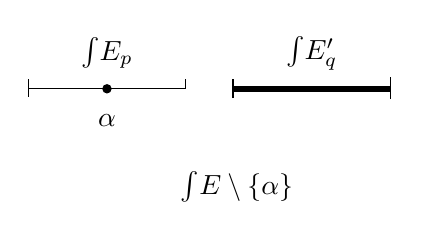
\begin{tikzpicture}[x=1cm,y=1cm]
\draw (0,0)--(2,0);\draw (0,-.10)--(0,.12);\draw (2,0)--(2,.13);\fill (1,0) circle (.06);
\node at (1,.45) {$\unsure{\int}E_p$};\node at (1,-.40) {$\alpha$};
\draw[line width=2pt] (2.6,0)--(4.6,0);\draw (2.6,-.12)--(2.6,.12);\draw (4.6,-.13)--(4.6,.15);
\node at (3.6,.45) {$\unsure{\int}E'_q$};
\node at (2.65,-1.25) {$\unsure{\int}E\setminus\{\alpha\}$};
\end{tikzpicture}}
\margin{$\unsure{p\geq}$}
\margin{278}

\deleted{
\[
F=\varinjlim_{A/F}\alpha\qquad G=\varinjlim_{A/G}\beta
\]
\[
\begin{aligned}
F\times G&=\varinjlim_{A/F}\underbrace{\alpha\times G}_{\varinjlim_{A/G}\alpha\times\beta}\\
&=\varinjlim_{A/F\times A/G}\alpha\times\beta
\end{aligned}
\]
\margin{$\alpha-F\qquad\beta-G$}
\[
\boxed{\begin{gathered}
\varphi_!(F\times G)=\varinjlim_{A/F\times A/G}
\underbrace{\varphi_!(\alpha\times\beta)}_{\varphi_!(\alpha)\times\varphi_!(\beta)}\\
\varphi_!(F)=\varinjlim_{A/F}\varphi_!(\alpha)\\
\varphi_!(G)=\varinjlim_{A/G}\varphi_!(\beta)
\end{gathered}}
\]
\diagram{\begin{tikzcd}[ampersand replacement=\&]
A\arrow[r,dash,"\varphi"]\&\mathcal X
\end{tikzcd}}
\diagram{\begin{tikzcd}[ampersand replacement=\&]
C=\mathcal X\arrow[r,shift right=2,"\unsure{u}=\varphi^*"']\&C'=\widehat A\arrow[l,shift right=2,"\unsure{v}=\varphi_!"']
\end{tikzcd}}
\figure{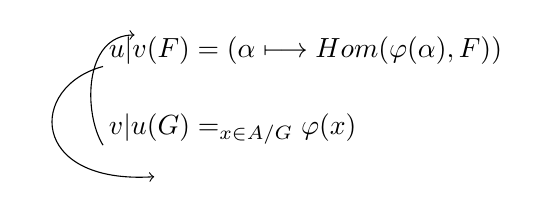
\begin{tikzpicture}
\node[anchor=west] at (0,0) {$\unsure{u|v}(F)=(\alpha\longmapsto\operatorname{Hom}(\varphi(\alpha),F))$};
\node[anchor=west] at (0,-1) {$\unsure{v|u}(G)=\varinjlim_{x\in A/G}\varphi(x)$};
\draw[->] (.05,-.2)..controls(-.9,-.45)and(-.9,-1.7)..(.7,-1.6);
\draw[->] (.05,-1.2)..controls(-.2,-.8)and(-.2,.2)..(.45,.2);
\end{tikzpicture}}
\margin{$u$ continu\\$v$ cocontinu}
\diagram{\begin{tikzcd}[ampersand replacement=\&,row sep=small]
\mathcal X\arrow[r]\&\widehat A\\
Y\&/\;a_i\to\varphi^*(Y)
\end{tikzcd}}
\diagram{\begin{tikzcd}[ampersand replacement=\&]
\varphi(a_i)\arrow[r]\&Y
\end{tikzcd}}
}

\margin{17}
\scanpage{19}
\mspage{\textcircled{2}}

\begin{center}
\uline{ACADEMIE D'AIX-MARSEILLE}\\
INSPECTION ACADEMIQUE\\
\uline{DE VAUCLUSE}
\end{center}

\diagram{\begin{tikzcd}[ampersand replacement=\&,column sep=small,row sep=small]
I\arrow[r,"\text{épi}"]\arrow[dr,"\text{épi}"']\&J\arrow[r,dash]\arrow[dr,dash,bend right]\&{}\\
\&K\&{}
\end{tikzcd}}
$\operatorname{card} I,J,K\leq3$

\diagram{\begin{tikzcd}[ampersand replacement=\&]
I\arrow[r]\arrow[d]\&J\arrow[r]\arrow[d]\&J'\arrow[d]\\
K\arrow[r]\&\unsure{\bullet|K'}\arrow[r,dash]\&\bullet
\end{tikzcd}}
\diagram{\begin{tikzcd}[ampersand replacement=\&]
X_0\&X_1\arrow[l]\&X_2\arrow[l]\\
X'_0\arrow[u]\&X'_1\arrow[l]\arrow[u,dash]\&X'_2\arrow[l,dash]\arrow[u]
\end{tikzcd}}

\diagram{\begin{tikzcd}[ampersand replacement=\&]
I\arrow[r,hook]\arrow[d]\&J=I\amalg K\arrow[d,dash]\\
I'\arrow[r,hook]\&J'=I'\amalg K
\end{tikzcd}}
\diagram{\begin{tikzcd}[ampersand replacement=\&,column sep=large]
X(\unsure{I})\&\begin{gathered}\deleted{X(I)\times X(K)}\\X(I\amalg K)\end{gathered}\arrow[l]\\
X(\unsure{I'})\arrow[u]\&X(I'\amalg K')\arrow[l]\arrow[u]
\end{tikzcd}}

\diagram{\begin{tikzcd}[ampersand replacement=\&]I\arrow[r]\&{}\end{tikzcd}}
\diagram{\begin{tikzcd}[ampersand replacement=\&]
\mathbb E_n\arrow[r,"\delta_n"]\arrow[d,"K_{n-1}"']\&\mathbb E_{n+1}\\
\mathbb E_n\&{}
\end{tikzcd}}
\deleted{$\unsure{u}$}

\figure{\begin{tikzpicture}
\node at (0,0) {\diagram{\begin{tikzcd}[ampersand replacement=\&,column sep=small,row sep=small]
\mathbb E_n\arrow[r,"\delta_n"]\arrow[d,"\delta_n"']\&\mathbb E_{n+1}\arrow[d]\\
\mathbb E_{n+1}\arrow[r]\&\mathbb E_{n+2}
\end{tikzcd}}};
\node at (2.6,0) {$n\geq1$};\node[draw,circle] at (3.65,.8) {II};
\node at (0,-2.6) {\diagram{\begin{tikzcd}[ampersand replacement=\&,column sep=small,row sep=small]
\mathbb E_n\arrow[r,"\delta_n"]\arrow[d,"K_{n-1}"']\&\mathbb E_{n+1}\arrow[d]\\
\mathbb E_{n-1}\arrow[r]\&\mathbb E_n
\end{tikzcd}}};
\node at (2.6,-2.6) {$n\geq2$};\node[draw,circle] at (3.65,-2.7) {III};
\draw (-2,-4)..controls(-1.6,-3.6)and(-1.4,-4.2)..(-1,-3.9)..controls(0,-4.2)and(1,-3.7)..(2,-4)..controls(2.5,-4.2)and(2.8,-3.8)..(3.2,-4);
\node at (0,-5.2) {\diagram{\begin{tikzcd}[ampersand replacement=\&,column sep=small,row sep=small]
\mathbb E_{n\deleted{\unsure{*}}}\arrow[r,"K_{n-1}"]\arrow[d,"K'_{n-1}"']\&\mathbb E_{n-1}\arrow[d,dash,"\deleted{\unsure{\alpha}}"]\\
\mathbb E_{n-1}\arrow[r,dash,"\deleted{\unsure{\alpha}}"]\&\mathbb E_{n-2}
\end{tikzcd}}};
\node at (2.6,-5.2) {$n\geq3$};\node[draw,circle] at (3.65,-4.8) {IV};
\node at (0,-7.8) {\diagram{\begin{tikzcd}[ampersand replacement=\&,column sep=small,row sep=small]
\mathbb E_n\arrow[r,"K_{n-1}"]\arrow[d,"K''_{n-1}"']\&\mathbb E_{n-1}\arrow[d]\\
\mathbb E_{n-1}\arrow[r]\&\mathbb E_{n-2}
\end{tikzcd}}};
\node at (2.6,-7.8) {$n\geq4$};\node[draw,circle] at (3.65,-7.7) {V};
\draw (-2.2,.3)..controls(-2.7,2.2)and(2.4,2)..(3.5,.8)..controls(4.3,-1)and(4,-4)..(4.1,-6)..controls(4.4,-8)and(3.9,-9)..(2.8,-9.3);
\end{tikzpicture}}

\figure{\begin{tikzpicture}
\node at (0,0) {\diagram{\begin{tikzcd}[ampersand replacement=\&,column sep=small,row sep=small]
\mathbb E_p\arrow[d]\&{}\\
\mathbb E_{p+q}\&\mathbb E_q\arrow[l]
\end{tikzcd}}};
\node[draw,circle] at (.3,1.4) {I};\node at (1.8,.6) {$p,q\geq1$};
\draw (-1.7,1.2)..controls(-.2,2)and(2.7,1.8)..(2.7,.2)..controls(2.7,-1.9)and(-.4,-2)..(-1.6,-.8)..controls(-2,-.5)and(-1.9,.4)..(-1.7,1.2);
\end{tikzpicture}}

\diagram{$\boxed{\begin{array}{clc}
\mathrm I&p=q=1&2\\
&p=1,q=2&\\
\mathrm {II}&n=1,\deleted{\unsure{2}}&1\\
\mathrm {III}&n=2,\deleted{\unsure{3}}&1\\
\mathrm {IV}&n=3&1\\
\mathrm V&&0
\end{array}}$}
\margin{$\unsure{*}$}

\diagram{$\boxed{\begin{array}{clc}
\mathrm I'&p=1,q=3&2\\
&p=2,q=2&\\
\mathrm {II}&n=2&1\\
\mathrm {III}&n=3&1\\
\mathrm {IV}&n=4&1\\
\mathrm V&n=4&1
\end{array}}$}

\deleted{
\diagram{\begin{tikzcd}[ampersand replacement=\&]
\unsure{\mathbb E'}\arrow[r]\&\unsure{\mathbb E'}
\end{tikzcd}}
\diagram{\begin{tikzcd}[ampersand replacement=\&]{}\arrow[r]\&{}\end{tikzcd}}
\figure{\begin{tikzpicture}\draw (0,0)--(.7,0);\draw(0,-.1)--(0,.1);\draw(.7,-.1)--(.7,.1);\node at (.35,.4) {$2$};\end{tikzpicture}}
\diagram{\begin{tikzcd}[ampersand replacement=\&]
\mathbb E^2\&\unsure{\mathbb E}\arrow[l,dash]\\
\mathbb E'\arrow[u,dash]\arrow[r,equals]\&\mathbb E'\arrow[u,dash]
\end{tikzcd}}
\diagram{\begin{tikzcd}[ampersand replacement=\&]
X^2\&X_1\arrow[l]\\
X_{\unsure{1|0}}\arrow[u]\arrow[r,equals]\&X_1\arrow[u,"1"']
\end{tikzcd}}
\figure{\begin{tikzpicture}\draw (0,0)--(.7,0);\draw(0,-.1)--(0,.1);\draw(.7,-.1)--(.7,.1);\end{tikzpicture}}
}

\margin{18}
\scanpage{20}
\mspage{\textcircled{3}}

\begin{center}
\uline{ACADEMIE D'AIX-MARSEILLE}\\
INSPECTION ACADEMIQUE\\
\uline{DE VAUCLUSE}
\end{center}

\diagram{\begin{tikzcd}[ampersand replacement=\&,column sep=large,row sep=small]
{}\&\unsure{\mathfrak S_2|\mathcal G_2}\&\unsure{\mathfrak S_3|\mathcal G_3}\\
X_1\arrow[r,bend right=55,"\delta_0"']\&X_2\arrow[l,shift right=1.2,"p_0"']\arrow[l,shift left=1.2,"p_1"]\arrow[r,bend right=45,"\delta_1"']\arrow[r,bend right=60,"\delta_2"']\arrow[r,bend right=75,"\delta_3"']\&X_3\arrow[l,shift right=3,"p_{12}"']\arrow[l,"p_{23}"']\arrow[l,shift left=3,"p_{31}"]
\end{tikzcd}}
\margin{$\rho,\sigma_1,\sigma_2,\sigma_3$}
\deleted{$p=q$}

\figure{\begin{tikzpicture}
\node at (0,0) {\diagram{\begin{tikzcd}[ampersand replacement=\&,column sep=large,row sep=large]
X_2\arrow[r,two heads,"{(p_0,p_1)\ \text{épi}}"]\&X_1\times X_1\\
{}\&X_1\arrow[u,hook]\arrow[ul,"\delta_0"']
\end{tikzcd}}};
\node at (-2.6,.5) {$\unsure{\mathfrak S_2|\mathcal G_2}$};
\node at (.15,1.5) {$\begin{gathered}p_0\sigma\\\Vert\end{gathered}$};
\draw (-1.8,1.65)--(2.1,1.8)..controls(2.5,1.8)and(2.5,1.8)..(2.5,1.3);\draw(2.5,1.1)--(2.7,-.15)..controls(2.7,-.4)and(2.3,-.4)..(-1.8,-.5);\draw(-1.8,-.5)--(-1.8,.9);
\node at (-1.6,-2) {iso ???};\draw (-1.6,-2) ellipse (1 and .5);
\draw[->] (-.3,.3)..controls(-.8,-.8)and(-2.8,-1.4)..(-2.3,-1.85);
\end{tikzpicture}}

\diagram{\begin{tikzcd}[ampersand replacement=\&,column sep=large]
X_3\arrow[r,two heads,"{(p_{12},\unsure{q_3})\ \text{épi}}"]\&X_2\times X_1\arrow[r,two heads,"{(p_0,p_1)\times\mathrm{id}_{X_1}}"]\&X_1\times X_1\times X_1
\end{tikzcd}}
\diagram{\begin{tikzcd}[ampersand replacement=\&,column sep=large]
X_3\arrow[r,two heads,"\text{épi}","{(p_{12},p_{23})}"']\&\overset{(p_1)}{X_2}\times_{X_1}\overset{(p_0)}{X_2}\arrow[r,two heads,"\text{épi}"]\&X_2\times_{X_1}(X_1\times X_1)
\end{tikzcd}}

\diagram{\begin{tikzcd}[ampersand replacement=\&]
\mathbb E_1\arrow[r]\arrow[d]\&\mathbb E_2\arrow[d]\\
\mathbb E_2\arrow[r]\&\mathbb E_3
\end{tikzcd}}
\figure{
\begin{tikzpicture}
\fill (0,0) circle (.04);\fill(.5,0) circle(.04);\fill(1,0)circle(.04);
\draw(0,-.18)..controls(.05,-.35)and(.2,-.35)..(.25,-.23)..controls(.35,-.35)and(.5,-.35)..(.5,-.18);
\draw(.5,.16)..controls(.55,.35)and(.7,.35)..(.75,.23)..controls(.85,.35)and(1,.35)..(1,.16);
\end{tikzpicture}}
\diagram{\begin{tikzcd}[ampersand replacement=\&]
\mathbb E_3\arrow[r,"K_2"]\arrow[d,"K'_2"']\&\mathbb E_2\arrow[d,"K_1"]\\
\mathbb E_2\arrow[r,"K_1"]\&\mathbb E_1
\end{tikzcd}}

\figure{\begin{tikzpicture}
\node at (0,0) {\diagram{\begin{tikzcd}[ampersand replacement=\&,column sep=large,row sep=large]
X_3\arrow[r,two heads,"\unsure{p_1|\delta_1}"]\&X_2\\
X_{\unsure{2}}\arrow[u,hook,"\delta_3"]\arrow[ur,phantom,"\text{cart}"]\&X_1\arrow[l,hook,"\delta_0"]\arrow[u,hook,"\delta_0"']
\end{tikzcd}}};\draw (0,0) ellipse (2.9 and 1.9);
\end{tikzpicture}}

\diagram{\begin{tikzcd}[ampersand replacement=\&]
\mathbb E_2\arrow[r,dash,"\delta_{\unsure{3|2}}"]\arrow[d,"K_{\unsure{1}}"']\&\mathbb E_3\arrow[d,"K'_2"]\\
\mathbb E_1\arrow[r,"\delta_1"]\&\mathbb E_2
\end{tikzcd}}

\deleted{\figure{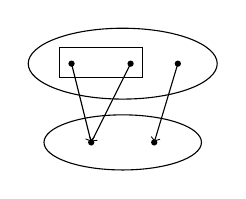
\begin{tikzpicture}
\draw(0,0)ellipse(1.2 and .45);\draw(-.8,-.18)rectangle(.25,.20);\fill(-.65,0)circle(.04);\fill(.1,0)circle(.04);\fill(.7,0)circle(.04);
\draw(0,-1)ellipse(1 and .35);\fill(-.4,-1)circle(.04);\fill(.4,-1)circle(.04);
\draw[->](-.65,0)--(-.4,-1);\draw[->](.1,0)--(-.4,-1);\draw[->](.7,0)--(.4,-1);
\end{tikzpicture}}}
\figure{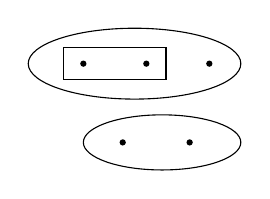
\begin{tikzpicture}
\draw(0,0)ellipse(1.35 and .45);\draw(-.9,-.2)rectangle(.4,.2);\fill(-.65,0)circle(.04);\fill(.15,0)circle(.04);\fill(.95,0)circle(.04);
\draw(.35,-1)ellipse(1 and .35);\fill(-.15,-1)circle(.04);\fill(.7,-1)circle(.04);
\end{tikzpicture}}
\deleted{\figure{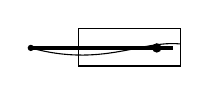
\begin{tikzpicture}
\draw[very thick](-.7,0)--(1.1,0);\fill(-.7,0)circle(.04);\fill(.9,0)circle(.06);\draw(-.1,-.23)rectangle(1.2,.25);\draw(-.7,0)..controls(.2,-.25)and(.7,.1)..(1.2,.05);
\end{tikzpicture}}}

\figure{\begin{tikzpicture}
\node at (0,0) {\diagram{\begin{tikzcd}[ampersand replacement=\&,column sep=large,row sep=large]
X_2\&X_3\arrow[l,"p_{12}"']\\
X_1\arrow[u,hook,"K_1"]\arrow[ur,phantom,"\text{cart}"]\&X_2\arrow[l,"\delta_1"]\arrow[u,hook,"K'_2"']
\end{tikzcd}}};\draw(0,0)ellipse(2.8 and 1.65);
\end{tikzpicture}}

\diagram{\begin{tikzcd}[ampersand replacement=\&,column sep=large,row sep=small]
{}\&\unsure{\mathfrak S_2|\mathcal G_2}\&\unsure{\mathfrak S_3|\mathcal G_3}\\
X_1\arrow[r,shift right=1.5,"K_1^*"']\&\deleted{X_2}\arrow[l,shift right=1.5,"\delta_1^*"']\arrow[r,shift right=1.5,"K_2^*"']\&X_3\arrow[l,shift right=1.5,"\delta_2^*"']
\end{tikzcd}}
\figure{\begin{tikzpicture}\draw(0,.45)--(0,0)--(1.6,0);\end{tikzpicture}}

\deleted{$\unsure{E}$}
Supposons $X_1$ réduit à un élément, donc $X_2$ est un $\unsure{\mathfrak S_2|\mathcal G_2}$-ens. à pt fixe marqué $\delta_2$, $X_3$ un $\unsure{\mathfrak S_3|\mathcal G_3}$-ens. à pt fixe marqué $\delta_3$
\diagram{\begin{tikzcd}[ampersand replacement=\&]
X_2\arrow[r,shift left,"\delta_2"]\&X_3\arrow[l,shift left,"K_2"]
\end{tikzcd}}
\deleted{$\unsure{\delta}$} $\delta_2$ et $K_2$ compatibles avec les \deleted{\unsure{pts fixes}} \unsure{structures|ponctuations} par $\delta_2,\delta_3$, avec
\[
K_2\delta_2=\mathrm{id}_{X_2}.
\]

\diagram{\begin{tikzcd}[ampersand replacement=\&]
\mathbb E_1\arrow[r,hook]\&\mathbb E_2\arrow[l,bend left=45]
\end{tikzcd}}
\figure{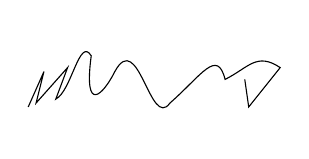
\begin{tikzpicture}
\draw(0,0)--(.2,.45)--(.1,.05)--(.5,.5)--(.35,.1)..controls(.55,.2)and(.65,.9)..(.8,.65)..controls(.7,-.1)and(.95,.15)..(1.1,.45)..controls(1.4,1)and(1.55,-.3)..(1.8,.05)..controls(2.2,.4)and(2.4,.75)..(2.5,.35)..controls(2.8,.5)and(2.9,.7)..(3.2,.5)--(2.8,0)--(2.75,.35);
\end{tikzpicture}}

\margin{19}
\scanpage{21}

\[
\unsure{\zeta|\xi}=(x,y)\qquad d\sigma(\unsure{\zeta|\xi})=(y,x,\unsure{x|n})
\]
\[
\rho^2d(\unsure{\zeta|\xi})=(y,x,y)
\]

\margin{20}
\scanpage{22}
\mspage{\textcircled{4}}

\begin{center}
\uline{ACADEMIE D'AIX-MARSEILLE}\\
INSPECTION ACADEMIQUE\\
\uline{DE VAUCLUSE}
\end{center}

\deleted{$\unsure{\mathfrak S}$}
\[
\unsure{\mathfrak S_2|\mathcal G_2}=\{1,\sigma\}\qquad
\unsure{\mathfrak S_3|\mathcal G_3}=\{1,\rho,\rho^2,\sigma_1,\sigma_2,\sigma_3)
\]
\margin{$[\rho^3=1,\inserted{\sigma_i^2=1,}\rho\sigma_i\rho^{-1}=\sigma_{i+1}\quad(\sigma_4=\sigma_1)]$}

\diagram{\begin{tikzcd}[ampersand replacement=\&,row sep=small,column sep=large]
X_1\arrow[d,phantom,"\Vert"]\&X_2\arrow[d,phantom,"\ni" rotate=90]\arrow[r,shift left,"d"]\&X_3\arrow[l,shift left,"p"]\arrow[d,phantom,"\ni" rotate=90]\\
\{e_1\}\&e_2\&e_3
\end{tikzcd}}
\[
\sigma e_2=e_2
\]
\margin{$-$}

\[
d(x,y)=(x,y,y)\qquad\rho d(x,y)=(y,y,x)\qquad\rho^2d(x,y)=(y,x,y)
\]
\[
p(x,y,z)=(x,y)
\]
\[
\begin{aligned}
\rho(x,y,z)&=(y,z,x)\\
\rho^2(x,y,z)&=(z,x,y)\\
\sigma_1(x,y,z)&=(x,z,y)\\
\sigma_2(x,y,z)&=(z,y,x)\\
\sigma_3(x,y,z)&=(y,x,z)
\end{aligned}
\]
\[
\boxed{\begin{aligned}
pd&=\mathrm{id}_{X_2}\\
p\rho d&=c\quad\text{application constante de valeur }e_2\\
p\rho^2d&=\sigma\\
\sigma_1d&=d\\
p\sigma_3&=\sigma p
\end{aligned}}\qquad\textcircled{*}
\]

\[
\unsure{\mathfrak S_3|\mathcal G_3}
=\deleted{\unsure{\{1,\rho,\rho^2\}}}\{1,\sigma_1\}\cdot\{1,\rho,\rho^2\}
=\underbrace{\{1,\rho,\rho^2\}}_g\cdot\underbrace{\{1,\sigma_1\}}_h.
\]
\[
d(X_2)\subset X_3\qquad(g\circ h)\circ d=g\circ d
\]
\[
\begin{gathered}
[\rho^i d(\unsure{\zeta|\xi})=\rho^{i'}d(\unsure{\zeta'|\xi'})]
\ \substack{\overset{?}{\Longrightarrow}\\[-2pt]\Longleftarrow}\
[i\equiv i'\ (3),\ \unsure{\zeta|\xi}=\unsure{\zeta'|\xi'}]\\
\Updownarrow\\
[d(\unsure{\zeta'|\xi'})=\rho^{i\deleted{\unsure{'}}-i'}d(\unsure{\zeta|\xi})]
\end{gathered}
\]
\margin{ou $[\unsure{\zeta|\xi}=\unsure{\zeta'|\xi'}=e_2]$}

\[
d(\unsure{\zeta'|\xi'})=\rho^j d(\unsure{\zeta|\xi})
\left\{\begin{aligned}
&\text{si }j=0\quad\text{on a}\quad\unsure{\zeta'|\xi'}=\unsure{\zeta|\xi}\quad\unsure{\text{c.q.f.d.}}\\
&\text{si }j=1\quad\text{on a}\quad\unsure{\zeta'|\xi'}=p\rho d(\unsure{\zeta|\xi})=e_2\\
&\text{donc}\quad e_3=\rho d(\unsure{\zeta|\xi})\\
&\inserted{d(\unsure{\zeta'|\xi'})=d(e_2)}\\
&\text{donc}\quad d(\unsure{\zeta|\xi})=e_3\quad\text{donc}\\
&\deleted{\text{donc}\quad d(\unsure{\zeta|\xi})=e_3}\\
&\unsure{\zeta|\xi}=pd(\unsure{\zeta|\xi})=pe_3=e_2\\
&\text{donc}\quad\unsure{\zeta|\xi}=\unsure{\zeta'|\xi'}=e_2\\
&\text{si }j=2,\quad\unsure{\zeta'|\xi'}=p\rho^2d(\unsure{\zeta|\xi})=\sigma\unsure{\zeta|\xi}
\end{aligned}\right.
\]
\margin{$d\sigma(\unsure{\zeta|\xi})=\rho^2d(\unsure{\zeta|\xi})\qquad d(\unsure{\zeta|\xi})=\rho d\sigma(\unsure{\zeta|\xi})$
\[
\unsure{\zeta|\xi}=p\rho d\sigma(\unsure{\zeta|\xi})=e_2,\quad\unsure{\zeta'|\xi'}=e_2
\]}

\margin{21}
\scanpage{23}
\mspage{5}

Ainsi, le sous-$\unsure{\mathfrak S_3|\mathcal G_3}$-ens. \inserted{$X'_3$} de $X_3$ engendré par $d(X_2)$ a une unique orbite à 1 \unsure{élémt}, savoir $\{e_3\}=\{de_2\}$, toutes les autres orbites sont de cardinal 3 \deleted{et} (avec la représentation régulière de $\unsure{\mathfrak S_3|\mathcal G_3}$), et elles sont en corr. biunivoque avec les éléments de $X_2\setminus\{e_2\}\overset{\mathrm{def}}=X_2^*$. Comme $\unsure{\mathfrak S_3|\mathcal G_3}$-ens $X'_3$ s'écrit canoniquement
\[
X'_3\simeq\{e_3\}\amalg\left(\unsure{\mathfrak S_3|\mathcal G_3}\wedge_{\{1,\sigma_1\}}X_2^*\right),
\]
où $\{1,\sigma_1\}$ opère trivialement sur $X_2^*$.

\margin{Et on a une explicitation de $p$ sur $X'_3$ via les trois premières des cinq formules $(*)$, \unsure{le reste} à satisfaire \unsure{étant} \unsure{formel} \unsure{par ces trois formules} \unsure{cas}.}

Reste à exprimer
\[
X_3^*\overset{\mathrm{def}}=X_3\setminus\underbrace{X'_3}_{\unsure{\mathfrak S_3|\mathcal G_3}\cdot d(X_2)}
\]
comme $\unsure{\mathfrak S_3|\mathcal G_3}$-ens, et l'application induite par $p$
\diagram{\begin{tikzcd}[ampersand replacement=\&]
X_3^*\arrow[r,two heads,"p^*=p\mid X_3^*"]\&X_2
\end{tikzcd}}
satisfaisant à
\[
\boxed{p^*\sigma_3=\sigma p^*}.
\]

\diagram{\begin{tikzcd}[ampersand replacement=\&]
X_3\arrow[r,two heads,"{p,p\rho}"]\&X_2\times X_2
\end{tikzcd}}
épi

\margin{$p(x,y,z)=(x,y)$
\[
p'(x,y,z)=(y,z)=p\rho(x,y,z)
\]}

pour $\unsure{\zeta|\xi},\eta\in X_2$, $\exists\alpha\in X_3$ avec
\[
p\alpha=\unsure{\zeta|\xi},\quad p\rho\alpha=\eta
\]

\margin{22}
\scanpage{24}
\mspage{\textcircled{6}}

\begin{center}
\uline{ACADEMIE D'AIX-MARSEILLE}\\
INSPECTION ACADEMIQUE\\
\uline{DE VAUCLUSE}
\end{center}

Quelle est la partie de $X_2\times X_2$ qui provient de $X'_3$ ?

\[
\text{a)}\quad(p,p\rho)(e_3)=(e_2,e_2)
\]
\[
\text{b)}\quad(p,p\rho)\underbrace{\rho^i d(\unsure{\xi|\zeta})}_{\substack{i\in\mathbb Z/3\mathbb Z\\\unsure{\xi|\zeta}\in X_2^*=X_2\setminus\{e_2\}}}
=\begin{cases}
(\unsure{\xi|\zeta},e_2)&\text{si }i=0\\
(e_2,\sigma\unsure{\xi|\zeta})&\text{si }i=1\\
(\sigma\unsure{\xi|\zeta},\unsure{\xi|\zeta})&\text{si }i=2
\end{cases}
\]

Donc on trouve les éléments \deleted{de la forme} dans
\[
\uline{\underbrace{(X_2\times\{e_2\})}_{\Sigma_1}\cup\underbrace{(\{e_2\}\times X_2)}_{\Sigma_2}\cup\deleted{\unsure{\Delta}}\Delta'}
\]
où $\Delta'$ est l'image de
\diagram{\begin{tikzcd}[ampersand replacement=\&]
X_2\arrow[r,"{\delta'=(\sigma,\mathrm{id}_{X_2})}"']\&X_2\times X_2
\end{tikzcd}}

\uline{NB} Cette partie $\Sigma$ de $X_2\times X_2$ est la réunion de $\Sigma_1,\Sigma_2,\Delta'$, et l'intersection de deux \unsure{quelconques} des trois est égale à $\{(e_2,e_2)\}$.

Quand a-t-on $\Sigma=X_2\times X_2$ ?

\deleted{\unsure{Si}} On a
\[
X_2\times X_2\setminus\{\Sigma_1\cup\Sigma_2)=X_2^*\times X_2^*,
\]
donc il est \unsure{nécs.} que $X_2^*\longrightarrow X_2^*\times X_2^*$ soit surj., i.e. que pour $\unsure{\zeta|\xi},\eta\in X_2^*$, on ait tjs $\eta=\sigma\unsure{\zeta|\xi}$. Cela signifie que l'on est dans l'un des 2 cas suivants

a) $X_2^*=\varnothing$ i.e. $X_2=\{e_2\}$

b) $X_2^*$ de cardinal 1 (donc $\sigma$ \deleted{\unsure{y}} y opère \unsure{trivialt})

\margin{i.e. $X_2$ de cardinal 2, (et $\sigma$ y opère \unsure{trivialt})}

[Si $X_2^*$ est de cardinal $\geq2$, alors s'il y a une seule orbite sous $\sigma$, celle-ci est de cardinal 2, et \deleted{$\unsure{\xi}$} $\forall\unsure{\zeta|\xi}\in X_2^*$, $(\unsure{\zeta|\xi},\unsure{\zeta|\xi})\notin\operatorname{Im}\delta'$ i.e. $\unsure{\zeta|\xi}\ne\sigma\unsure{\zeta|\xi}$). S'il y a \deleted{\unsure{donc}} au moins deux orbites, on prend $\unsure{\zeta|\xi},\eta$ dans deux orbites différentes, et on a bien $\eta\ne\sigma\unsure{\zeta|\xi}$.

\margin{23}
\scanpage{25}
\mspage{\textcircled{7}}

\margin{$X_2=\{e_2,\unsure{\zeta|\xi})$}
Supposons \inserted{donc} $X_2$ de cardinal 2, \deleted{\unsure{donc}} et \deleted{\unsure{que}} $X_3=X'_3$ donc
\[
X_3=\{e_3\}\amalg\{d\unsure{\zeta|\xi},\rho d\unsure{\zeta|\xi},\rho^2d\unsure{\zeta|\xi}\},
\]
considérons les deux carrés

$(*)$
\diagram{\begin{tikzcd}[ampersand replacement=\&,column sep=large,row sep=large]
X_3\arrow[r,"{\delta_1=d=((x,y)\longmapsto(x,y,y))}"]\&X_2\arrow[d,dash,"\delta_0"]\\
X_2\arrow[u,"\delta_3"]\arrow[r,"\delta_0"]\&X_1=\{e_1\}
\end{tikzcd}}

et

$(**)$
\diagram{\begin{tikzcd}[ampersand replacement=\&,column sep=large,row sep=large]
X_2\&X_3\arrow[l,"p=p_{12}"']\\
\begin{gathered}X_1\\\{e_1\}=\end{gathered}\arrow[u,"{K_1=\delta_0\deleted{\unsure{K}}}"]\&X_2\arrow[l,"p_1"]\arrow[u,"{K'_2=((x,y)\longmapsto(x,x,y))}"']
\end{tikzcd}}
\inserted{$(=\delta_3)$}.

sont-ils cartésiens ? On a $\delta_3(x,y)=(x,x,y)\deleted{\unsure{=}}$,
\[
\deleted{d\sigma(x,y)}\quad d\sigma(x,y)=d(y,x)=(y,x,x)=\deleted{\unsure{\rho}}\rho^2\delta_3(x,y)
\]
i.e. $\delta_3=\rho^{\deleted{\unsure{2}}}d\sigma$. Donc en général (supposant seulement $\operatorname{card}X_1=1$ i.e. $X_1=\{e_1\}$), \deleted{\unsure{et quand}} \unsure{pour les}, quand a-t-on, \inserted{pour $\unsure{\zeta|\xi},\unsure{\zeta'|\xi'}\in X_2$,}
\[
d(\unsure{\zeta|\xi})=\rho^{\deleted{\unsure{2}}}d\underbrace{\sigma(\unsure{\zeta'|\xi'})}_{\unsure{\zeta''|\xi''}}\quad ?
\]
Il faut \unsure{s.} qu'on ait \deleted{\unsure{alors}}
$\unsure{\zeta|\xi}=\unsure{\zeta''|\xi''}=e_2$, \deleted{donc} $\boxed{\text{OK}}$.
\margin{d'où $\unsure{\zeta'|\xi'}=e_2$}

\deleted{$\unsure{\zeta|\xi}=\unsure{\zeta'|\xi'}=e_2$ \unsure{ce}} cas est bien cartésien, sans autre hypothèse. Le cas \unsure{$(**)$} s'écrit
\[
p_{\deleted{\unsure{12}}}^{-1}(e_2)\overset{?}=\delta_3(X_2)\quad[=\rho d\sigma(X_2)=\rho d(X_2)]
\]
\deleted{Mais $\unsure{p_{31}(x,y,z)}=\unsure{(z,x)}=\unsure{p\rho^2(x,y,z)}$ \unsure{i.e.} $\unsure{p_{31}=p\rho^2}$,}
\deleted{\unsure{puis}} i.e.
\[
p^{-1}(e_2)\overset{?}=\rho d(X_2)\qquad(\text{on a a priori }\supset)
\]
Si $X_3=X'_3\overset{\mathrm{def}}=\unsure{\mathfrak S_3|\mathcal G_3}\cdot d(X_2)$,
\deleted{\unsure{alors un objet de} $\unsure{X_3}$}
\inserted{\unsure{l'on est ramené à}}
\deleted{$X'_3$ \unsure{s'écrit}} prouvons que \deleted{\unsure{donc}} si $\unsure{\zeta|\xi}\in X'_3\setminus\{e_3\}$ satisfait à $p(\unsure{\zeta|\xi})=e_2$, on a $\unsure{\zeta|\xi}\in\rho d(X_2)$. Or $\unsure{\zeta|\xi}$ s'écrit canoniquement
\[
\unsure{\zeta|\xi}=\rho^i d(\eta),\quad\text{avec }\eta\in X_2^*,\quad\text{et }i\in\{0,1,2\},
\]
et on a
\[
p\unsure{\zeta|\xi}=\begin{cases}
\eta\ (\ne e_2)&\text{si }i=0\\
\sigma\eta\ (\ne e_2)&\text{si }\unsure{i=1|i=2}
\end{cases}
\]
\deleted{$\unsure{(p\sigma_3d)(x,y)}=\unsure{p\rho d(x,y)}=\unsure{\mathrm{id}}$}
donc $p\unsure{\zeta|\xi}=e_2\Longrightarrow i=1$, Qed.

\margin{24}
\scanpage{27}
\mspage{1}

\uline{Structures stratifiées.}

1. \uline{La situation la plus élémentaire}, en un sens qui apparaîtra, sera la suivante. On se donne des espaces (disons !) en attendant que \unsure{ça|ce} devienne des topos\ldots)

(1)
\diagram{\begin{tikzcd}[ampersand replacement=\&]Y\arrow[r,hook]\&X\end{tikzcd}}

$Y$ fermé dans $X$. On suppose que la ``structure normale\unsure{''} de $X$ le long de $Y$ soit loc. triviale''\unsure{)}, i.e. que pour tout $y\in Y$, existe un voisinage ouvert $X'$ de $y$ \unsure{et} un espace $Z$ pointé par $z$, et un diagramme commutatif (où $Y'=Y\cap X'$)

(2)
\diagram{\begin{tikzcd}[ampersand replacement=\&,column sep=large,row sep=large]
Y'\arrow[r,hook]\arrow[d,"\text{can}"',"\sim"]\&X'\arrow[d,"\sim"]\\
Y'\times\{z\}\arrow[r,hook,"\mathrm{id}_{Y'}\times i_{z,Z}"']\&Y'\times Z
\end{tikzcd}}

où $X'\simeq Y'\times Z$ est un homéomorphisme.

On considère alors ``le voisinage tubulaire'' (``infinitésimal'') de $Y$ dans $X$, soit

(3)
\diagram{\begin{tikzcd}[ampersand replacement=\&]
Y\arrow[r,hook]\&\unsure{\mathcal V_{Y,X}|V_{Y,X}}\arrow[r,hook]\&X
\end{tikzcd}},

dont il faudra donner une définition

\margin{26}
\scanpage{28}

techniquement simple. Si $X$ est un \deleted{\unsure{paracompact}} espace paracompact, on pourra prendre (à titre provisoire !) pour $\unsure{\mathcal V_{Y,X}|V_{Y,X}}$ le ``germe d'espaces'' de $X$ autour de $Y$ -- qui est donc un topos, sav. la $\varprojlim$ toposique des voisinages ouverts de $Y$ dans $X$. Intuitivement, $\unsure{\mathcal V_{Y,X}|V_{Y,X}}\hookrightarrow X$ a les propriétés d'une imm. ouverte, et $Y\hookrightarrow\unsure{\mathcal V_{Y,X}|V_{Y,X}}$ celles d'une immersion fermée, et (3) constitue une factorisation canonique de (1).

\deleted{L'hypothèse de locale trivialité normale implique que l'on a (moyennant des conditions de ``modération'' convenables) une inclusion}

\margin{L'intérêt principal de cette factorisation, c'est que \unsure{l'inclusion} $Y\longrightarrow\unsure{\mathcal V_{Y,X}|V_{Y,X}}$ est une ``équivalence d'homotopie'' (indépendamment de toute hyp. de locale trivialité).}

(4)
\diagram{\begin{tikzcd}[ampersand replacement=\&]
Y\arrow[r,"\text{équi. d'homotopie}"]\&\unsure{\mathcal V_{Y,X}|V_{Y,X}}
\end{tikzcd}}

Supposons p. ex. $Y$ et $X-Y=X^*$ des variétés, et $Z\inserted{{}^*=Z\setminus\{z\}}$ une variété (moyennant des hyp. de modération, l'hyp. sur $Z$ devrait être une conséquence de la première hypothèse), \deleted{\unsure{et que}} alors que $z$ est un pt singulier \inserted{de $Z$}, i.e. $X$ est ``singulier le long de $Y$''. Il est naturel alors de vouloir reconstruire $X$ en termes des variétés $Y$ et $X^*$,

\margin{27}
\scanpage{29}
\mspage{2}

jouant le rôle de ``pierres de construction'' élémentaires. Ceci amène à introduire
\[
(5)\qquad \unsure{\mathcal V_{Y,X}^*|V_{Y,X}^*}\overset{\mathrm{déf}}=\unsure{\mathcal V_{Y,X}|V_{Y,X}}\cap X^*=\unsure{\mathcal V_{Y,X}|V_{Y,X}}\setminus Y
\]
\[
(X^*=X-Y),
\]
et le diagramme \deleted{\unsure{un}}

(6)
\diagram{\begin{tikzcd}[ampersand replacement=\&,column sep=large]
\unsure{\mathcal V_{Y,X}^*|V_{Y,X}^*}\arrow[r,hook,"\substack{\text{bouchage de trous}\\\text{le long de }Y}"]\arrow[d]\&\unsure{\mathcal V_{Y,X}|V_{Y,X}}\arrow[d]\\
X^*\arrow[r]\&X
\end{tikzcd}}

Je vais regarder (indépendamment de toute hypothèse de locale trivialité normale, ou de lissité de $X^*$ et $Y$) $X$ comme obtenu par \uline{recollement} de $\unsure{\mathcal V_{Y,X}|V_{Y,X}}$ et de $X^*$ suivant leur intersection $\unsure{\mathcal V_{Y,X}^*|V_{Y,X}^*}$, ou (en termes plus techniques) comme la somme amalgamée, ou comme \deleted{\unsure{espace}} espace-topos $\varinjlim$ du diagramme

(7)
\diagram{\begin{tikzcd}[ampersand replacement=\&]
\unsure{\mathcal V_{Y,X}^*|V_{Y,X}^*}\arrow[r,hook]\arrow[d]\&\unsure{\mathcal V_{Y,X}|V_{Y,X}}\\
X^*\&
\end{tikzcd}}

\margin{28}
\scanpage{30}

Si on dispose d'une théorie suffisamment souple des types d'homotopie, on devrait pouvoir en déduire le type d'homotopie de $X$ comme ``somme amalgamée'' des types d'homotopie des trois \deleted{topos}\inserted{``espaces''} $\unsure{\mathcal V_{Y,X}^*|V_{Y,X}^*}$, $\unsure{\mathcal V_{Y,X}|V_{Y,X}}$ et $X^*$ (dont les deux premiers sont de nature ``infinitésimale''). Par exemple, on doit avoir pour les \unsure{espaces} déduits en ``tuant les $\pi_i$ pour $i\geq2$'' -- donc, essentiellement, pour les groupoïdes fondamentaux, un ``théorème de van Kampen'', qui s'exprime par le fait que le diagramme des groupoïdes fondamentaux

(8)
\diagram{\begin{tikzcd}[ampersand replacement=\&,column sep=small]
\Pi_1\unsure{\mathcal V_{Y,X}^*|V_{Y,X}^*}\arrow[rr,"p"]\arrow[d,"i"']\&\&\Pi_1\unsure{\mathcal V_{Y,X}|V_{Y,X}}\ (\xleftarrow{\sim}\Pi_1Y)\arrow[d,dotted]\\
\Pi_1X^*\&\bigl(\arrow[r,dotted]\&\Pi_1X\ \bigr)
\end{tikzcd}}

\margin{29}
\scanpage{31}
\mspage{3}

est cocartésien -- ou encore, si $Y,X,X^*$ sont connexes, et qu'on choisit un ``pt base'' de $\Pi_1\unsure{\mathcal V_{Y,X}^*|V_{Y,X}^*}$ (i.e. par définition, un rev. universel de $\unsure{\mathcal V_{Y,X}^*|V_{Y,X}^*}$) (d'où des pts bases de $\Pi_1\unsure{\mathcal V_{Y,X}|V_{Y,X}}$, \deleted{\unsure{et un point} de $\Pi_1X^*)$}\inserted{$\Pi_1X^*,\Pi_1X)$}, qu'on a un isom. \inserted{\unsure{can.}} de groupes fondamentaux
\[
(9)\qquad \unsure{\pi|\Pi}_1(X)\simeq\unsure{\pi|\Pi}_1(X^*)\wedge_{\unsure{\pi|\Pi}_1\unsure{\mathcal V_{Y,X}^*|V_{Y,X}^*}}\underbrace{\unsure{\pi|\Pi}_1(\unsure{\mathcal V_{Y,X}|V_{Y,X}})}_{\simeq\unsure{\pi|\Pi}_1(Y)},
\]
où $\unsure{\pi|\Pi}_1(\unsure{\mathcal V_{Y,X}|V_{Y,X}})$ est isom. \inserted{\unsure{extérieurem\textsuperscript{t}}} à $\unsure{\pi|\Pi}_1(Y)$.

\deleted{\unsure{relatif} à un pt base choisi de}

Pour expliciter $\unsure{\pi|\Pi}_1(X)$ en termes des données ``élémentaires'', \deleted{il reste} dont $\unsure{\pi|\Pi}_1(Y)$ \inserted{et} $\unsure{\pi|\Pi}_1(X^*)$, \deleted{et} il \unsure{resterait} encore à expliciter la structure de $\unsure{\pi|\Pi}_1(\unsure{\mathcal V_{Y,X}^*|V_{Y,X}^*})$, qui s'envoie dans l'un et dans l'autre, donnant lieu justement au diagramme

\margin{\unsure{cette flèche définie moy\textsuperscript{t}} d'un choix suppl. (pt base de $Y$ et classe de chemins de $x$ vers $y$)}

(10)
\diagram{\begin{tikzcd}[ampersand replacement=\&]
\unsure{\pi|\Pi}_1(\unsure{\mathcal V_{Y,X}^*|V_{Y,X}^*})\arrow[r]\arrow[d]\&\unsure{\pi|\Pi}_1(\deleted{\unsure{X}}Y)\\
\unsure{\pi|\Pi}_1(X^*)\&
\end{tikzcd}}

qui exprime (8). C'est ici que l'hypothèse

\margin{30}
